
\documentclass[9pt, landscape]{article}
\usepackage[english]{babel}
\usepackage[utf8]{inputenc}
\usepackage[document]{ragged2e}
\usepackage[landscape]{geometry}       
\geometry{a4paper}
\geometry{margin=0.4in} 
\usepackage{paralist,sectsty,multicol,multirow,hyperref,titlesec,caption}
  \sectionfont{\small}
  \subsectionfont{\small}
  \titlespacing*{\section}
  {0pt}{3pt}{1pt}
  \titlespacing*{\subsection}
  {0pt}{1.8pt}{1pt}
\hypersetup{
    colorlinks=true,
    linkcolor=blue,
    filecolor=magenta,      
    urlcolor=cyan,
}
\newlength{\mylen}
\setbox1=\hbox{$\bullet$}\setbox2=\hbox{\tiny$\bullet$}
\setlength{\mylen}{\dimexpr0.5\ht1-0.5\ht2}
\renewcommand\labelitemi{\raisebox{\mylen}{\tiny$\bullet$}}

% ---------------------------------------------------------------
% Math Basics
% ---------------------------------------------------------------
\usepackage{enumitem}
\setlist[itemize]{leftmargin=0pt}
\usepackage{bbm, bm}
\usepackage{amsmath, amssymb, amsthm, mathrsfs, mathtools,stmaryrd}
\usepackage{booktabs, tikz, array, eurosym, float, makecell}
\DeclareMathOperator*{\argmax}{argmax}
\DeclareMathOperator*{\argmin}{argmin}

% ---------------------------------------------------------------
% Code Blocks
% ---------------------------------------------------------------
\usepackage{algorithm,algorithmicx}
\usepackage[noend]{algpseudocode}
\captionsetup[algorithm]{font=footnotesize}
\newcommand{\commentsymbol}{$\sslash$}
\algrenewcommand\algorithmiccomment[1]{\hfill \commentsymbol{} #1}

\newcommand{\boxwidth}{246pt}
\newcommand\disteq{\stackrel{\mathclap{\normalfont\mbox{\tiny d}}}{=}}
\pagenumbering{gobble}
% ---------------------------------------------------------------

% ---------------------------------------------------------------
% Geometric figures
% ---------------------------------------------------------------
\usepackage{tkz-euclide}
\usetkzobj{all}
% ---------------------------------------------------------------

\begin{document}    
\footnotesize


\begin{multicols*}{3}
\section{Brain Teasers}
\begin{itemize}
	\item \textbf{Information Encoding:} The type of problems ask to represent \& discern different states of a system using numbers/bits. $k^{n}$ states can be represented by $n$ $k$-ary digits: say, 00, 01, 10, 11 for 4 states.
	\begin{itemize}[leftmargin=10pt,noitemsep,topsep=0pt,partopsep=0pt]
		\item[-] \textbf{\href{https://math.stackexchange.com/questions/639/logic-problem-identifying-poisoned-wines-out-of-a-sample-minimizing-test-subje}{1000 Wine Bottles}:} \textit{The system has 1000 states, live/die of one tester is a bit of information. So we need $\left \lceil{\log_2 N}\right \rceil$. Extension with $k$ poison bottles is suprisingly much more complex.}
		\item[-] \textbf{\href{https://puzzling.stackexchange.com/questions/183/twelve-balls-and-a-scale/224\#224}{12 Balls and a Balance}:} Find the defect ball (heavier or lighter) with 3 measurements. 
		\textit{Analysis: (1) For single measurement of a heavier ball, 3-way operation $\{L, R, \emptyset\}$ corresponds to the 3 outcome states. (2) $3^3$ outcomes to discern $12\times 2$ results.} 
		\begin{center}
		\tiny
		\setlength{\tabcolsep}{3pt}
		\begin{tabular}{ |c|c|c|c|c|c|c|c|c|c|c|c|c|c| } 
		 \hline
		 \multirow{3}{*}{\makecell{Operation on Ball $i$ \\ in 3 measurememts}}& 
		  L& & &L& &R&L& &R&R&L&R \\ 
		 & &R& &L&L& &R&L& &R&R&L \\ 
		 & & &R& &L&R& &R&L&L&L&R \\ 
		 \hline
		 Ball $i$ is heavier & $1$ & $2$ & $3$ & $4$ & $5$ & $6$ & $7$ & $8$ & $9$ & $10$ & $11$ & $12$ \\
		 \hline
		\end{tabular}
		\end{center}
		\textit{The operations read: $1,4,7,11|6,9,8,10$, ... Flip the outcome sign to map to the 12 lighter ball cases.}
		\item[-] \textbf{Weighing Coins I:} 5 bags each has 100 coins  (10g), except 1 bag has fake coins (11g). Find it with 1 weighing on digital scale. \\
		\textit{The system has 5 states, so the outcome should take at least 5 different values. Take $i$ coins from the $i$-th bag, total weight = 15 coins $\times$ 10 grams + $i$ grams = $150+i$}.
		\item[-] \textbf{Weighing Coins II:} Each bag may have fake coins (11g). Follow-up: fake coins can be 9 or 11g.\\
		\textit{There are $2^5$ states. Draw $2^{k-1}$ coins from the $k$-th bag. \\}
		\textit{Allowing $-1$ as an extra individual state, the system now has $3^5$ states. Draw $3^{k-1}$ coins from the $k$-th bag.}
		\item[-] \textbf{\href{https://math.stackexchange.com/questions/446130/quickest-way-to-determine-a-polynomial-with-positive-integer-coefficients}{Identify Polynomial}:} Function $p(x)$ computes value of a polynomial of unknown order and \textit{non-negative integer} coefficients wrt. $x$, identify the polynomial coefficients with minimal calls of $p$.
		\textit{First time: $z = p(1) = \sum_{j=0}^{n} a_j$, we'll know all $0<a_j \leq z$ and the order $n\leq z-1$. Second time: $M = p(z+1) = \sum_{j=0}^{z-1} a_j (z+1)^j$. Do a base$(z+1)$ expansion of number $M$, the results are $\{a_j\}$'s.} 
		\item[-] \textbf{Hat Colors I:} $N$ people wearing R/B hats, called sequentially to declare the color of his hat and everyone else can hear it. Maximize \# of correct declarations. \\
		\textit{Suppose the first person sees $(N_R, N_B)$. He encodes $C_1 = N_B \% 2$ with R/B and says it. Anyone $k$ has own code $C_k = N_B\%2$ or $(N_B-1)\% 2$. So $k$ in red if $C_k=C_1$, else blue.}
		\item[-] \textbf{Hat Colors II:} There are $m$ different colors. \\
		\textit{Encode $C_1 = \{\sum_{i=1}^m  (i-1) N_i\} \% m = S_1\%m$ with $m$-colors. Anyone wearing color $j$ sees $N_j-1$ in that color, hence the code $C_k= \{\sum_{i\ne j} (i-1) N_i + j(N_j - 1)\} \% m = (S_1 - j)\%m, j\in [0, m-1]$.}
	\end{itemize}
	\item \textbf{\href{https://en.wikipedia.org/wiki/Pigeonhole_principle}{Pigeonhole Principle}:} $mn+1$ items to put in $n$ containers, at least 1 has $m+1$ items. 
	\begin{itemize}[leftmargin=10pt,noitemsep,topsep=0pt,partopsep=0pt]
		\item[-] \textbf{Handshake:} 10 ppl and I at the party, each shook hands with me, then at least 2 shook same number of hands. \\
		\textit{Each shook 1-25 hands (holes), and there are 26 ppl (pigeons). }
		\item[-] \textbf{Friend Circle:} there are 6 people at the party, either at least 3 are friends (with each other), or at least 3 are strangers.\\
		\textit{There are 1-6 friend circles. (3-6): 3 strangers by selecting 1 from each circ. (1-2): 6 pigeons in 1/2 holes, at least 3 friends.}.
	\end{itemize}
	\item \textbf{Summation:} $\sum_{k=1}^n k^2 = n(n+1)(2n+1)/6$. $\sum_{k=0}^{n-1} a_0 q^{k} = a_0\frac{1-q^n}{1-q}$
	\begin{itemize}[leftmargin=10pt,noitemsep,topsep=0pt,partopsep=0pt]
		\item[-] \textbf{Missing 2 Integers:} \textit{Sum $k$ and $k^2$, solve 2 equations.}
		\item[-] \textbf{\href{http://datagenetics.com/blog/july22012/index.html}{Two Eggs}:} Given 2 eggs, find the $n$-th floor where the eggs starts to break. Minimize worst case \#throws.\\
		\textit{Assume $x$ throws in total. Drop E1 at $x$-th floor; if it breaks, try E2 from $1,2,...,(x-1)$; if not, Drop B1 at $x+(x-1)$ since only $x-2$ drops left for E2. Worst case: $x+(x-1)+...+2+1\geq 100$}.\\
		Follow ups - 100 eggs: binary search. k eggs: see the DP section.
	\end{itemize}
	\item \textbf{\href{https://en.wikipedia.org/wiki/Induction_puzzles}{Multi-Agenet Induction}:}
	\begin{itemize}[leftmargin=10pt,noitemsep,topsep=0pt,partopsep=0pt]
	\item[-] \textbf{Flip Glass:} \textit{Green Book pp.17.} $n$ men get summoned randomly, can filp the Glass (initially $0$) or don't. At some point, a man can correctly identify everyone has been summoned at least once. \\
	\textit{The man who make the call (``Counter''): $1\to 0, 0\to 0$. Everyone else: $0\to 1, 1\to 1$, do nothing if he has fliped once.}
	\end{itemize}
	\item \textbf{\href{https://en.wikipedia.org/wiki/Mathematical_induction}{Mathematical Induction}:}
	\begin{itemize}[leftmargin=10pt,noitemsep,topsep=0pt,partopsep=0pt]
		\item[-] \textbf{Coin Split:} Recursively split $n$ coins into 2 piles until all piles has 1 coin. Find $S_n$ = $\sum_{i \in \{\text{all splits}\}} x_{i1} x_{i2}$. \\
		\textit{Claim: $S_n = S_{n-1} + n-1 = n(n-1)/2$, $\forall n = 2,...,N$. \\
		Consider $\forall k=1,...,N$}: $S_{N+1} = S_{k}+S_{N+1-k} +k(N+1-k) = k(k-1)/2 + (N+1-k)(N-k)/2 + k(N+1-k)= N(N+1)/2$. 
		\item[-] \textbf{Chocolate Bars:} Number of splits needed to break $m\times n$ chocolate bar into $1\times1$ pieces. \\
		\textit{Hack: number of pieces += 1 for each break, so $1+S_{mn}=mn$.} \textit{Induction Claim: $S_{mn}=mn-1, \forall m \leq M, n\leq N$, show for $S_{M+1, N}$ and $S_{M, N+1}$}
	\end{itemize}
	\item \textbf{\href{https://en.wikipedia.org/wiki/Kelly_criterion}{Kelly Criterion}:} Two-outcomes bet with a $p$ probability to win: (1) lose all bet, (2) win a fixed proportion (payoff odds, $\alpha$) of the bet. Optimal strategy is to bet a fixed fraction of current wealth, $f$. \\
	$f^* = \argmax~(1+\alpha f)^{p}(1-f)^{1-p}$, take log. $f^*= (\alpha p + p - 1) / \alpha$. \\
	General case: $f^* = \argmax~(1+\alpha f)^{p}(1-\beta f)^{q}$, $f^*= p/\beta - q/\alpha$.
	\item \textbf{Miscellaneous:}
	\begin{itemize}[leftmargin=10pt,noitemsep,topsep=0pt,partopsep=0pt]
		\item[-] \textbf{Horse Race:} Find 3 fastest horses out of 25 with fewest races, each race can have at most 5 horses.
		{\setlength\multicolsep{0.5pt}
		\begin{multicols*}{2}
		\textit{Let the following matrix be the ordering of the horses:}
		{\scriptsize$$
		\begin{pmatrix}
			\color{red}{1} & \color{orange}{2} & \color{blue}{3} & 4 & 5 \\
			\color{orange}{6} & \color{blue}{7} & 8 & 9 & 10 \\
			\color{blue}{11} & 12 & 13 & 14 & 15 \\
			16 & 17 & 18 & 19 & 20 \\
			21 & 22 & 23 & 24 & 25 \\
		\end{pmatrix}
		$$}
		\textit{First run 5 races row-wise, then run the 6-th race along first column. Now 1 has to be 1st; 2,6 are possible for 2nd-place; 3,7,11 for 3rd. 7-th race among 2,6,3,7,11.}
		\end{multicols*}}
		\item[-] \textbf{Hat Colors III:} 7 ppl randomly assigned 7 colors (can be duplicates), \textit{guess simultaneously}, s.t. at least one correct guess.
	\end{itemize}
\end{itemize}

\section{Calculus}
\begin{itemize}
	\item \textbf{\href{https://en.wikipedia.org/wiki/Convergent_series}{Convergent Series} \& \href{https://en.wikipedia.org/wiki/Convergence_tests}{Tests}:} 
	\begin{itemize}[leftmargin=10pt,noitemsep,topsep=0pt,partopsep=0pt]
		\item[-] \textbf{Integral Test:} The \href{https://en.wikipedia.org/wiki/Harmonic_series_(mathematics)}{\textit{Harmonic series}} diverges: Sum of rectanngles $\sum_{i=1}^n \frac{1}{k} > \int_1^{n+1} \frac{1}{x} dx = \log (n+1) \to \infty$. 
		\item[-] \textbf{Comparison Test:} $\sum_{k=1}^{n} \frac{1}{k^2}$ convergent. $\frac{1}{k^2} < \frac{1}{k(k-1)}$. Hence $\sum_{k=2}^n \frac{1}{k} < \sum_{k=2}^n (\frac{1}{k-1} - \frac{1}{k}) = 1-\frac{1}{n} \to 1$.
	\end{itemize}
\end{itemize}

\section{Linear Algebra}
\subsection{Fundamental Subspace, \href{https://en.wikipedia.org/wiki/Determinant}{Det}, \href{https://en.wikipedia.org/wiki/Invertible_matrix}{Invertibility}, etc}
\begin{itemize}
	\item For $n\times n$ square matrix $\bm{A}$, the following statements are equivalent (TFAE), i.e. they are \textit{either all True or all False for any given $\bm{A}$}:
	\begin{itemize}[leftmargin=10pt,noitemsep,topsep=0pt,partopsep=0pt]
		\item[-] $\bm{A}$ is invertible, $\bm{Ax} = \bm{b}$ has exactly one solution in $\mathbb{R}^n$.
		\item[-] $\bm{A}$ has full rank, the columns of $\bm{A}$ are linearly \textbf{in}dependent.
		\item[-] $\text{Ker}(\bm{A})$ is trivial, i.e. $\bm{Ax} = \bm{0}$ has only solution $\bm{x}=\bm{0}$.
		\item[-] $\text{det}(A) \ne 0$, $\bm{A}$ doesn't have 0 eigenvalue.
		\item[-] $\text{span}\{\text{Col}(\bm{A})\} = \mathbb{R}^n$.
	\end{itemize}
	\item \textbf{\href{https://en.wikipedia.org/wiki/Trace_(linear_algebra)}{Trace}:} Sum of eigenvalues, \textit{Cyclic property: }$\text{tr}(\bm{ABC}) = \text{tr}(\bm{BCA}) = \text{tr}(\bm{CAB}) \ne \text{tr}(\bm{ACB})$.
\end{itemize}
\subsection{\href{https://en.wikipedia.org/wiki/Eigenvalues_and_eigenvectors}{Eigenvalues and Eigenvectors}}
Square matrix $\bm{A}$: $\bm{Av} = \lambda \bm{v}$. $\lambda$ is eigval of $\bm{A}$ $\iff$ it's a root of the characteristic polynomial $P_{\bm{A}}(t) = \det( t \bm{I} - \bm{A})$, i.e. $\lambda$ solves $\det(\lambda \bm{I} - \bm{A}) = 0$
\begin{itemize}
	\item 
	\item \textbf{Some Puzzles}
	\begin{itemize}[leftmargin=10pt,noitemsep,topsep=0pt,partopsep=0pt]
		\item[-] \textbf{Eigvals of Self-Outerproduct:} $\bm{A} = \bm{v}\bm{v}^{\top}$. Notice that: $\bm{Av} = \bm{v}\bm{v}^{\top} \bm{v} = (\bm{v}^{\top} \bm{v}) \bm{v}$. So $\bm{v}^{\top} \bm{v}$ is eigval that corresponds to eigvec $\bm{v}$. Also: $\text{tr}(\bm{v}\bm{v}^{\top}) = \text{tr}(\bm{v}^{\top} \bm{v}) = \bm{v}^{\top} \bm{v}$ which is sum of all eigvals $\Rightarrow$ $0$ is eigval with multiplicity $n-1$, none zero $\bm{v}^{\top} \bm{v}$ has multiplicity $1$.
	\end{itemize}
\end{itemize}
\begin{itemize}
	\item \textbf{\href{https://en.wikipedia.org/wiki/Moore-Penrose_inverse}{Pseudoinverse}:} $\bm{X}\in \mathbb{R}^{m\times n}$ has full rank, $\bm{X}^{+} = (\bm{X}^{\top} \bm{X})^{-1} \bm{X}$ if $\bm{X}$ has linearly indep. cols; $\bm{X}^{+} = \bm{X}^{\top} (\bm{X}\bm{X}^{\top})^{-1}$ lindep. rows.
	\item \textbf{SVD:}
	\item \textbf{Covariance Matrix:} $\mathrm{\mathbb{C}ov}\left[\bm{X}\right] = \mathbb{E}\left[(\bm{X}- \mathbb{E}\left[\bm{X}\right])(\bm{X}- \mathbb{E}\left[\bm{X}\right])^{\top}\right]$.
\end{itemize}

\section{Optimization}
\begin{itemize}
	\item \textbf{\href{https://www.zhihu.com/question/23311674/answer/235256926}{KKT Conditions}:} 
	\item \textbf{Mean-Variance Problem:} $\max_{\bm{x}}~\bm{\mu}^{\top} \bm{x} - \frac{\gamma}{2} \bm{x}^{\top} \bm{\Sigma} \bm{x}$, $s.t.~\bm{1}^{\top} \bm{x} = 1$. 
	$$
	\bm{x}^* =  \frac{\lambda}{\bm{1}^{\top} \bm{\Sigma}^{-1} \bm{\mu}} \bm{\Sigma}^{-1} \bm{\mu} + \frac{1- \lambda}{\bm{1}^{\top} \bm{\Sigma}^{-1} \bm{1}} \bm{\Sigma}^{-1} \bm{1};~\text{where }\lambda=\frac{\bm{1}^{\top} \bm{\Sigma}^{-1}\bm{\mu}}{\gamma}
	$$
\end{itemize}


\section{Stochastic Models}
\subsection{Puzzles}
\begin{itemize}
	\item \textbf{Mutually Exclusive, Collectively Exhaustive Events}
	\begin{itemize}[leftmargin=10pt,noitemsep,topsep=0pt,partopsep=0pt]
	 	\item A filps $n+1$ coins, B filps $n$ coins. $\mathbb{P}\left(\text{A has more heads}\right)$?\\
	 	\textit{A filps the first $n$ coins. $\{\text{A more heads}\}$, $\{\text{A less heads}\}$, $\{\text{Equal}\}$ MECE}. $2p_1 + p_2 = 1$. $\mathbb{P}\left(E\right) = p_1 + p_2/2 = 1/2$.
	 	\item 52 cards, draw 2 without replacement. $\mathbb{P}\left(\text{1st} > \text{2nd}\right)$?\\
	 	\textit{$2p+p_{tie} = 1$}. $p_{tie} = \frac{13C1 \times 4C2}{52C2} = 1/17$. $p=8/17$.
	 	\item \textbf{\href{https://math.stackexchange.com/questions/5595/taking-seats-on-a-plane?noredirect=1&lq=1}{Taking Seat on Plane}:}  100 Seats. Person \#1 is drunk. $\mathbb{P}\left(\text{Person \#100 gets his seat}\right)$.\\
	 	\textit{Say $k$'s seat is occupied, equal prob to take seat \#1 or \#100. If $k$ takes \#1, all after $k$ gets own seat; if \#100, the last person will have to take seat \#1. $\mathbb{P}=1/2$.}
	 \end{itemize} 
	\item \textbf{Russian Roulette} \textit{(Green Book pp.81)} Single bullet in the gun, be the first or second? $\mathbb{P}\left(D|\text{First}\right) = \mathbb{P}\left(\text{bullet in 1,3,5 slot}\right) = 1/2$.
	\begin{itemize}[leftmargin=10pt,noitemsep,topsep=0pt,partopsep=0pt]
		\item[-] \textit{Spin} the revolver after each trial: $\mathbb{P}\left(D|\text{First}\right) = \frac{1}{6} + (\frac{5}{6})^2 \frac{1}{6} + (\frac{5}{6})^4 \frac{1}{6} + ... = \lim\limits_{n\rightarrow\infty} \frac{1}{6} \frac{1-(25/36)^n}{1-25/36} = \frac{6}{11}$. So we want to be the second player. Recursion solution: $\mathbb{P}\left(D|\text{First}\right) = \frac{1}{6} + (\frac{5}{6})^2 \mathbb{P}\left(D|\text{First}\right)$.
		\item[-] There are \textit{2 bullets} in the gun, I'm the second player. Opponent survived the first shot, should I spin or not? Obviously, $\mathbb{P}\left(D|\text{spin}\right) = \frac{1}{3}$. $\mathbb{P}\left(D|\text{not spin}\right) = \binom{4}{1} \binom{1}{1} \Big/ \binom{5}{2} = \frac{2}{5}$. Spin!
		\item[-] There are \textit{2 consecutive bullets} in the gun: $\mathbb{P}\left(D|\text{spin}\right) = \frac{1}{3}$ regardless of the positioning of the bullet. But $\mathbb{P}\left(D|\text{not spin}\right) = \frac{\{\text{Bullet at 2,3}\}}{\{\text{Consecutive bullets in 2,3,4,5,6}\}} = \frac{1}{4}$. Don't spin!
	\end{itemize}
	\item \textbf{Compute Probabilities by Conditioning.} 
	\begin{itemize}[leftmargin=10pt,noitemsep,topsep=0pt,partopsep=0pt]
		\item[-] \textbf{Extinction Problem:} A creature dies/stays same/spawn to 2/spawn to 3 with equal prob. $E = \{\text{Extinction}\}$. $\mathbb{P}\left(E\right) = \sum_{i=0}^3 \mathbb{P}\left(E | F_i\right) \mathbb{P}\left(F_i\right)$. Turns out that $\mathbb{P}\left(E|F_i\right)$ is equivalent to playing this game independently $i$-times (for $i$ offsprings), hence $\mathbb{P}\left(E|F_i\right) = \mathbb{P}\left(E\right)^i$. $\Rightarrow \mathbb{P}\left(E\right) = \frac{1}{4}(1+\mathbb{P}\left(E\right)+\mathbb{P}\left(E\right)^2 + \mathbb{P}\left(E\right)^3)$.
	\end{itemize}
	\item \textbf{Compute Expectation by Linearity.}
	\begin{itemize}[leftmargin=10pt,noitemsep,topsep=0pt,partopsep=0pt]
		\item[-] \textbf{\href{https://en.wikipedia.org/wiki/Coupon_collector's_problem}{Coupon Collection I}.} Equal probability to see any 1 of n different types of coupons, expected number of trials until seen all $n$ types. Let $X_k$ be number of trials to open to see a new type when $(k-1)$ types have already been collected $X_k\sim \text{Geometric}(\frac{n-(k-1)}{n})$. 
		{$$
		\mathbb{E}\left[X\right] = \sum_{k=1}^{n} X_k = \sum_{k=1}^n \tfrac{n}{n-(k-1)} = 1+\tfrac{n}{n-1}+\tfrac{n}{n-2} + ... + n
		$$}
	\end{itemize}
	\item \textbf{Compute Expectation by \href{https://en.wikipedia.org/wiki/Markov_chain}{Markov Chain}.} 
	\begin{itemize}[leftmargin=10pt,noitemsep,topsep=0pt,partopsep=0pt]
		\item[-]  \textbf{Coupon Collection II.}
	\end{itemize}
	\item \textbf{\href{https://en.wikipedia.org/wiki/Conditional_expectation}{Conditional Expectations}:} Properties: 
	\begin{itemize}[leftmargin=10pt,noitemsep,topsep=0pt,partopsep=0pt]
		\item[1.] \textbf{Pulling out independent factors:} If $X \perp \mathcal{F}$, then $\mathbb{E}\left[X\middle|\mathcal{F}\right] = \mathbb{E}\left[X\right]$. If $X \perp \sigma(Y, \mathcal{F})$, then $\mathbb{E}\left[XY\middle|\mathcal{F}\right] = \mathbb{E}\left[X\right] \mathbb{E}\left[Y\middle|\mathcal{F}\right]$, note that both independence to $Y$ and $\mathcal{F}$ are required.
		\item[2.] \textbf{Pulling out known factors:} If $\bm{X} \in m \mathcal{F}$, then $\mathbb{E}\left[XY\middle|\mathcal{F}\right] = X \mathbb{E}\left[Y\middle|\mathcal{F}\right]$; For RV $Y, Z$: $\mathbb{E}\left[f(Z) Y\middle|\sigma(Z)\right] = f(Z) \mathbb{E}\left[Y\middle|\sigma(Z)\right]$
	\end{itemize}
	\begin{itemize}[leftmargin=10pt,noitemsep,topsep=0pt,partopsep=0pt]
		\item[-] \textbf{Expectation of OLS beta:} Sample $(x_i, y_i)$ uniformly from region: $\{0 \leq x,y\leq1; x+y \geq 1.5\}$, and run OLS with intercept between sample $\bm{y}= \beta_0  + \beta_1\bm{x}$. Compute $\mathbb{E}[\widehat{\beta}_0], \mathbb{E}[\widehat{\beta}_1]$. Let $\bm{X} = (\bm{\iota}, \bm{x})$
		$$
		\mathbb{E}\left[\widehat{\beta} | \bm{X}\right] = \mathbb{E}\left[ (\bm{X}^{\top} \bm{X})^{-1} \bm{X}^{\top} \bm{y} | \bm{X} \right] = (\bm{X}^{\top} \bm{X})^{-1} \bm{X}^{\top} \mathbb{E}\left[\bm{y}\middle|\bm{X}\right]
		$$
		Turns out: $y_i | x_i = \frac{1}{2}(1+(\frac{3}{2}-x_i)) = \frac{5}{4} - \frac{1}{2}x_i$. $\mathbb{E}\left[\bm{y}\middle|\bm{X}\right] = \bm{X}(\frac{5}{4}, -\frac{1}{2})^{\top}$. $\bm{X}^{\top} \bm{X}$ cancels out, $\mathbb{E}[\widehat{\beta}_0, \widehat{\beta}_1] = \frac{5}{4}, -\frac{1}{2}$.
	\end{itemize}
\end{itemize}
\subsection{Measure space theory}
\begin{itemize}
	\item \textbf{Inequalities:} Pass
	\item \textbf{\href{https://en.wikipedia.org/wiki/Convergence_of_random_variables}{Convergence of RVs}:}
	\begin{itemize}[leftmargin=10pt,noitemsep,topsep=0pt,partopsep=0pt]
	\item[-] \textbf{Convergence In Prob / Almost Surely}: $X_n \xrightarrow{a.s.} X \iff \mathbb{P}\left( \lim_{n\rightarrow\infty}X_n = X \right) = 1$: \emph{the limit of $X_n(s)$ is $X$ with measure 1 wrt $s\in \Omega$, an anology of pointwise convergence in the measure space (SLLN).} $X_n \xrightarrow{p} X \iff \lim_{n\rightarrow\infty}\mathbb{P}\left(|X_n - X| > \epsilon \right) = 0, \forall \epsilon >0$: \textit{the probability of unusual outcome becomes smaller and smaller (Consistent estimator, WLLN).}
	\item \textbf{Convergence In Prob but not A.S.:} $X_1(\omega) = \mathbbm{1}(w\in[0, \tfrac{1}{2}]), X_2(\omega) = \mathbbm{1}(w\in[\tfrac{1}{2}, 1]), X_3(\omega) = \mathbbm{1}(w\in[0, \tfrac{1}{3}]), X_4(\omega) = \mathbbm{1}(w\in[\tfrac{1}{3}, \tfrac{2}{3}]), ..., \omega \sim \text{Uniform}[0, 1]$.
	\end{itemize}
\end{itemize}
\subsection{Named Distributions}
\begin{itemize}
	\item \textbf{\href{https://en.wikipedia.org/wiki/Normal_distribution}{Gaussian}:}
	\begin{itemize}[leftmargin=10pt,noitemsep,topsep=0pt,partopsep=0pt]
		\item[-] \textbf{Partition:} $\bm{x} = (\bm{x}_1; \bm{x}_2) \sim \mathcal{N}(\bm{\mu}, \bm{\Sigma})$, $\bm{\mu}= (\bm{\mu}_1; \bm{\mu}_2)$, $\bm{\Sigma} = (\bm{\Sigma}_{11}, \bm{\Sigma}_{12}; \bm{\Sigma}_{21}, \bm{\Sigma}_{22})$. Then $\bm{x}_1 | \bm{x}_2 \sim \mathcal{N}(\bm{\mu}_{\bm{x}_1|\bm{x}_2}, \bm{\Sigma}_{\bm{x}_1|\bm{x}_2})$, where $\bm{\mu}_{\bm{x}_1|\bm{x}_2} = \bm{\mu}_1 + \bm{\Sigma}_{12} \bm{\Sigma}_{22}^{-1} (\bm{x}_2 - \bm{\mu}_2)$; $\bm{\Sigma}_{\bm{x}_1|\bm{x}_2} = \bm{\Sigma}_{11}-\bm{\Sigma}_{12} \bm{\Sigma}_{22}^{-1} \bm{\Sigma}_{21}$. Marginal $\bm{x}_1 \sim \mathcal{N}(\bm{\mu}_1, \bm{\Sigma}_{11})$.
		\item[-] \textbf{Bayes Theorem:} Given $\bm{x}\sim \mathcal{N}(\bm{\mu}, \bm{\Gamma}), \bm{y}|\bm{x} \sim \mathcal{N}(\bm{A}\bm{x}+\bm{b}, \bm{\Omega})$. Then: $\bm{y}\sim \mathcal{N}(\bm{Ax}+\bm{b}, \bm{\Omega} + \bm{A}^{\top} \bm{\Gamma} \bm{A})$ \\
		$\bm{x}|\bm{y} \sim \mathcal{N}(\bm{\Sigma}[\bm{A}^{\top} \bm{\Omega}^{-1}(\bm{y}-\bm{b}) + \bm{\Gamma}^{-1}\bm{\mu}], \bm{\Sigma} )$, $\bm{\Sigma} = (\bm{\Gamma}^{-1} + \bm{A}^{\top} \bm{\Omega}^{-1} \bm{A})^{-1}$.
	\end{itemize}
	\item \textbf{\href{https://en.wikipedia.org/wiki/Chi-squared_distribution}{Chi-Squared}:}
	\begin{itemize}[leftmargin=10pt,noitemsep,topsep=0pt,partopsep=0pt]
		\item[-] \textbf{Quad Form:} If $m$-vector $\bm{x}\sim \mathcal{N}(\bm{0}, \bm{\Sigma})$, then $\bm{x}^{\top} \bm{\Sigma}^{-1} \bm{x} \sim \chi^2(m)$.
		\item[-] \textbf{Projection:} $n$-vector $\bm{z}\sim \mathcal{N}(\bm{0}, \bm{I})$, $\bm{P}$ is rank-$r$ projection matrix onto a subspace of $E^n$, then $\bm{z}^{\top} \bm{P} \bm{z} \sim \chi^2(r)$.
	\end{itemize}
	\item ss
\end{itemize}

\section{OLS}
\begin{itemize}
	\item \textbf{\href{https://en.wikipedia.org/wiki/Ordinary_least_squares\#Assumptions}{OLS Assumptions} And Their Purposes:}
	\begin{itemize}[leftmargin=10pt,noitemsep,topsep=0pt,partopsep=0pt]
		\item[-] \textbf{Linearity:} Correct specification of the linear functional form. 
		\item[-] \textbf{No Perfect Multicollinearity:} Assures the min-square problem has a unique solution (the linear system: FOC) - the $\widehat{\bm{\beta}}$ are identifiable.
		\item[-] \textbf{Exogeneity of $\bm{X}$:} $\mathbb{E}\left[\bm{u} | \bm{X}\right] = 0$. This allows us to derive $\mathbb{E}\left[\widehat{\bm{\beta}} - \bm{\beta}\right] = \mathbb{E}\left[(\bm{X}^{\top} \bm{X})^{-1} \bm{X}^{\top} \bm{u}\right] = 0$ (tower property), i.e. OLS estimator is \textit{unbiased}. \textbf{Relaxation:} Instrumental Variables.
		\item[-] \textbf{$\bm{X}$ has Finite Second Moment:} This means $\frac{1}{n} \bm{X}^{\top} \bm{X} \xrightarrow{p} \bm{S}_{\bm{X}^{\top} \bm{X}}$, i.e. converge in probability to a finite and positive semi-definite matrix $\bm{S}_{\bm{X}^{\top} \bm{X}}$. This is a much-used condition in deriving asymptotic properties, including all of the aymptotic tests and consistency.
		\item[-] \textbf{Error Term Distribution:} There are several versions, from strongest to weakest:
		\begin{itemize}[leftmargin=10pt,noitemsep,topsep=0pt,partopsep=0pt]
			\item[1.] \textbf{Normality:} $\bm{u} \sim \text{i.i.d. } \mathcal{N}(\bm{0}, \sigma^2 \bm{I})$. $\Rightarrow$ Finite sample statistical (exact) tests; and makes OLS equivalent to MLE.
			\item[2.] \textbf{Spherical Errors:} $\bm{u}$ follows some i.i.d. (not normal) distribution with equal variance. This allows asymptotic statistical tests, by applying CLT.
			\item[3.] \textbf{No Serial Correlation:} $\mathbbm{Cov}[\bm{u}|\bm{X}] = \text{diag}\{\sigma_k\}_1^n$. This corresponds to \href{https://en.wikipedia.org/wiki/Weighted_least_squares}{\textit{Weighted Least Squares}} and other Heteroskedasticity-Robust method.
			\item[4.] \textbf{(General) Deterministic Cov Matrix:} $\mathbbm{Cov}[\bm{u} | \bm{X}] = \bm{Omega}$, corresponds to \href{https://en.wikipedia.org/wiki/Generalized_least_squares}{\textit{Generalized Least Squares}}.
		\end{itemize}
	\end{itemize}
	\item \textbf{\href{https://en.wikipedia.org/wiki/Frisch-Waugh-Lovell_theorem}{FWL Theorem}:} $\bm{y} = \bm{X}_1 \bm{\beta}_1 + \bm{X}_2 \bm{\beta}_2 + \bm{u}$, $\bm{M}_1\bm{y} = \bm{M}_1 \bm{X}_2 \bm{\beta}_2 + \bm{u}$ has same ols estimator and residuals. $\widehat{\bm{\beta}}_2 = (\bm{X_2}^{\top} \bm{M_1}\bm{X_2})^{-1} \bm{X_2}^{\top} \bm{M}_1 \bm{y}$. $\bm{M}_1 \bm{y} = \bm{M}_1 \bm{X}_2 \widehat{\bm{\beta}}_2 + \bm{M}_1 \bm{M}_{\bm{X}} \bm{y}$ $\Rightarrow$ $\bm{M}_1 \bm{y} - \bm{M}_1 \bm{X}_2 \widehat{\bm{\beta}}_2 = \bm{M}_{\bm{X}} \bm{y}$. 
	\begin{itemize}[leftmargin=10pt,noitemsep,topsep=0pt,partopsep=0pt]
		\item[-] Adding $\bm{X}_2$ into $\bm{y} = \bm{X}_1 \bm{\beta}_1 + \bm{u}$ is likely to cause change in $\widehat{\bm{\beta}}_1$, won't if $\bm{M}_{\bm{X}_2} \bm{X}_1 = \bm{X}_1$ i.e. $\bm{X}_1 \perp \bm{X}_2$.
	\end{itemize}
	\item \textbf{\href{https://en.wikipedia.org/wiki/Coefficient_of_determination}{R Squared}: } Let $\bm{\iota}$ be column of $n$ ``1''s. Projecting $\bm{y}$ onto $\bm{\iota}$ yields a column of $n$ copies of the mean of $\bm{y}$. Easy to verify that $\bm{H}_{\iota}$ has $(n\times n)$ entries of $\frac{1}{n}$'s.
	$$
	R^2 = 1 - \frac{\text{SSRes}}{\text{SSTot}} = 1 - \frac{\sum_{i=1}^n (y_i - \widehat{y}_i)^2}{\sum_{i=1}^n (y_i - \bar{y})^2} = \frac{\bm{y}^{\top} (\bm{M}_{\bm{\iota}} - \bm{M}_{\bm{X}}) \bm{y}}{\bm{y}^{\top} \bm{M}_{\bm{\iota}} \bm{y}}
	$$
	\begin{itemize}[leftmargin=10pt,noitemsep,topsep=0pt,partopsep=0pt]
		\item[-] When $\bm{X}$ has intercept term, $R^2 \geq 0$ for sure, because $(\bm{M}_{\bm{\iota}} - \bm{M}_{\bm{X}})$ is symmetric-idempotent, thus positive-semidefinite. If no intercept, could be negative: extreme counter example: $y_i = 100 + \text{small } \epsilon_i$, $x_i=1,2,...$. 
		\item[-] $\bm{y} \sim \bm{x}_1$ yields $R_1^2$, $\bm{y} \sim \bm{x}_2$ yields $R_2^2$, what's the range of $R^2$ for $\bm{y} \sim \bm{x}_1 + \bm{x}_2$ (WLOG assume stuffs have mean 0). \\
		\textit{The answer is $R^2 \in [\max\{R_1^2, R_2^2\}, 1]$}. \textit{$R^2$ can actually be derived as a function of $\mathrm{\mathbb{C}orr}(\bm{x}_1, \bm{y})=R_1, \mathrm{\mathbb{C}orr}(\bm{x}_2, \bm{y})=R_2,$ and $\mathrm{\mathbb{C}orr}(\bm{x}_1, \bm{x}_2)=:\rho_{x_1, x_2}$ by the following geometric proof:}
		\begin{center}
		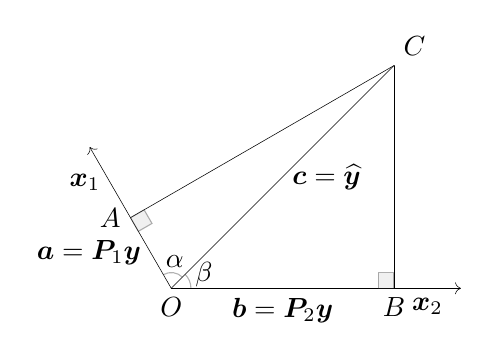
\begin{tikzpicture}
		\tkzDefPoint(0,0){O}
		\tkzDefPoint(2.8284,2.8284){C}
		\tkzDefPoint(-0.5176, 0.8966){A}
		\tkzDefPoint(-0.5176*2, 0.8966*2){A2}
		\tkzDefPoint(2.8284,0){B}
		\tkzDefPoint(1.3*2.8284,0){B2}

		\tkzDrawSegments(O,A O,B O,C A,C B,C)
		\tkzDrawSegments[arrows=->](A,A2 B,B2)
		\tkzLabelSegment[left](O,A){$\bm{a} = \bm{P}_1 \bm{y}$} 
		\tkzLabelSegment[left](A,A2){$\bm{x}_1$} 
		\tkzLabelSegment[below](O,B){$\bm{b} = \bm{P}_{2}\bm{y}$}
		\tkzLabelSegment[below](B,B2){$\bm{x}_2$} 
		\tkzLabelSegment[right](O,C){$\bm{c} = \widehat{\bm{y}}$} 
		\tkzMarkRightAngles[fill=black!20,size=.2,opacity=.3](O,A,C O,B,C)
		\tkzMarkAngle[fill=black!20,size=.2,opacity=.3](C,O,A)
		\tkzMarkAngle[fill=black!20,size=.25,opacity=.3](B,O,C)
		\tkzLabelAngle[pos=0.34](C,O,A){$\alpha$}
		\tkzLabelAngle[pos=0.45](B,O,C){$\beta$} 

		%\tkzMarkSegments[mark=s||](I,A I,B I,C I,D)
		\tkzLabelPoints[below](O,B) 
		\tkzLabelPoints[above right](C)  
		\tkzLabelPoints[left](A)
		\end{tikzpicture}
		\end{center} 
		{\scriptsize
		\begin{equation*}
			\begin{split}
			\rho_{x_1x_2} &= \cos(\alpha + \beta) = \cos \alpha \cos \beta - \sin \alpha \sin \beta \\
			&= \frac{ab}{c^2} - \sqrt{1-\frac{a^2}{c^2}} \sqrt{1-\frac{b^2}{c^2}}\\
			\Rightarrow \quad R^2 &= \frac{c^2}{y^2} = \frac{(a^2 + b^2 - 2ab \rho_{x_1x_2}) / y^2}{1-\rho_{x_1x_2}^2} = \frac{R_1^2 + R_2^2 - 2R_1R_2 \rho_{x_1x_2}}{1-\rho_{x_1x_2}^2}
			\end{split}
		\end{equation*}}
		Obvious that $R^2$ can be 1 when $\bm{y} \in \text{span}\{\bm{x}_1, \bm{x}_2\}$. $R^2 - R_1^2 \geq 0$ because that reduces to $\rho^2_{x_1x_2}R_1^2 + R_2^2 - 2\rho_{x_1x_2} R_1 R_2 = (\rho_{x_1x_2}R_1 - R_2)^2$. 
	\end{itemize}
	\item \textbf{{Misc Algebra Questions}:}
	\begin{itemize}[leftmargin=10pt,noitemsep,topsep=0pt,partopsep=0pt]
		\item[-] \textbf{Product of Projection Matrices:} If $\text{span}\{ \bm{X}_1 \} \subseteq \text{span} \{ \bm{X}\}$, then $\bm{P}_{\bm{X}} \bm{P}_{\bm{X}_1} = \bm{P}_{\bm{X}_1}$ (proj onto the smaller subspace); and $\bm{M}_{\bm{X}} \bm{M}_{\bm{X}_1} = \bm{M}_{\bm{X}}$ ($\perp$proj onto the bigger subspace).
		\item[-] \textbf{Zero $\bm{x}_2$ Coefficient:} $\bm{P}_1 \bm{y} = \widehat{\beta}_1 \bm{x}_1$, $\bm{P}_{\bm{X}} \bm{y} = \widehat{\beta}_1' \bm{x}_1 + 0 \bm{x}_2$. Premultiply both ols with $\bm{P}_1$, since $\bm{P}_1 \bm{P}_{\bm{X}} = \bm{P_{1}}$ (always, when $\bm{x}_1 \in \text{span}\{\bm{X}\}$) $\Rightarrow$ $\widehat{\beta}_1 = \widehat{\beta}'_1$. 
		\item[-] \textbf{\href{https://stats.stackexchange.com/questions/20553/effect-of-switching-response-and-explanatory-variable-in-simple-linear-regressio}{Exchange $\bm{x}, \bm{y}$}:} $\widehat{\beta}_{y\sim x} \widehat{\beta}_{x\sim y} = (\bm{x}^{\top} \bm{y})^2 / (\bm{x}^{\top} \bm{x}\cdot \bm{y}^{\top} \bm{y}) = \text{Corr}^2(\bm{x}, \bm{y}) \leq 1$. I.e. $\widehat{\beta}_{y\sim x} \leq 1/ \widehat{\beta}_{x\sim y}$.
		\item[-] \textbf{\href{https://stats.stackexchange.com/questions/216003/what-are-the-consequences-of-copying-a-data-set-for-ols}{Duplicate Data}:} $\mathrm{\mathbb{V}ar}[\widehat{\bm{\beta}}] = \frac{\sigma^2}{2} (\bm{X}^{\top} \bm{X})^{-1}$, underestimated, half of the correct value. $R^2, \bm{\widehat{\beta}}$ doesn't change. Implication is that correlation in $\bm{X}$ downplays the variance estimate.
		\item[-] \textbf{\href{https://stats.stackexchange.com/questions/2125/whats-the-difference-between-correlation-and-simple-linear-regression}{$\widehat{\bm{\beta}}$ and Correlation}:} For simple linear regression with intercept or without intercept while the RV $X, Y$ has 0 mean: $\widehat{\beta} = \mathrm{\mathbb{C}orr}\left[X,Y\right]$. \\
		\textit{Application:} For zero mean RVs $X_1, X_2, Y$, suppose $\rho_{X_1,Y}=0.1, \rho_{X_2,Y}=0.2$, run $\bm{y} \sim \bm{x}_1 + \bm{x}_2$, will $\widehat{\beta}_2$ be negative?
	\end{itemize}
	\item \textbf{Prediction Error:}
	\item \textbf{Leverage:} $(\widehat{\bm{\beta}}^{(t)} - \bm{\beta})$. Removing $t$-th obs = Adding unit basis $\bm{e}_t$ into the regression. $\bm{y} = \bm{X}\bm{\beta}' + \alpha \bm{e}_t + \bm{u}$, $\bm{M}_t\bm{y} = \bm{M}_t\bm{X}\bm{\beta}^{(t)} + \bm{u}$. \\
	$\bm{X}\widehat{\bm{\beta}} = \bm{H}_{\bm{X}}\bm{H}_{\bm{X},\bm{e}_t} \bm{y} = \bm{H}_{\bm{X}}(\bm{X}\widehat{\bm{\beta}}^{(t)} + \widehat{\alpha} \bm{e}_t)$. Hence $(\widehat{\bm{\beta}}^{(t)} - \widehat{\bm{\beta}}) = -\widehat{\alpha}(\bm{X}^{\top} \bm{X})^{-1} \bm{X}^{\top} \bm{e}_t = \frac{-\widehat{u}_t}{1-h_{tt}} (\bm{X}^{\top} \bm{X})^{-1} \bm{x}_t^{\top}$. (\textit{$\widehat{\alpha}$ obtained by another FWL: $\bm{M}_{\bm{X}}\bm{y} = \alpha\bm{M}_{\bm{X}}\bm{e}_t + \bm{u}$}, and $h_{tt} = \bm{e}_t^{\top} \bm{H}_{\bm{X}}\bm{e}_t = \cos^2 \langle \bm{e}_t, \bm{H}_{\bm{X}} \bm{e}_t \rangle$)
	\item \textbf{Hypothesis Testing:}
	\begin{itemize}[leftmargin=10pt,noitemsep,topsep=0pt,partopsep=0pt]
		\item[-] \textbf{\href{https://en.wikipedia.org/wiki/Student's_t-test}{T-Test}:} $\bm{y} = \bm{X}_1 \bm{\beta}_1 + \bm{x}_2 \beta_2 + \bm{u}$. $\bm{z}(\widehat{\beta}_2) = \widehat{\beta}_2 / \text{se}(\widehat{\beta}_2)  = \bm{x}_2^{\top} \bm{M}_1 \bm{y} / \sigma (\bm{x}_2^{\top}\bm{M}_1 \bm{x}_2)^{1/2} \sim \mathcal{N}(0,1)$ under the null hypothesis $\beta_2 = 0$; $\text{RSS} / \sigma^2 = \bm{y}^{\top} \bm{M}_{\bm{X}} \bm{y} / \sigma^2 \sim \chi^2(n-p)$, \textit{by the projection property of $\chi^2$}. The t-statistic for $\beta_2$:
		{\scriptsize$$
		t(\widehat{\beta}_2) = \frac{z(\widehat{\beta}_2)}{\sqrt{\chi^2_{n-p}/(n-p)}} = \frac{\bm{x}^{\top}_2 \bm{M}_1 \bm{y}}{\sigma(\bm{x}_2^{\top} \bm{M}_1 \bm{x}_2)^{\frac{1}{2}}} \left(\frac{RSS}{\sigma^2 (n-p)}\right)^{-\frac{1}{2}}
		$$}
		\item[-] \textbf{\href{https://en.wikipedia.org/wiki/F-test}{F-Test}:}
	\end{itemize}
	\item \textbf{\href{https://en.wikipedia.org/wiki/Regression_toward_the_mean}{Regression Toward the Mean (Mediocrity)}:} The son of a tall father is on average shorter than the father - closer to the human mean height. Consider the bivariate normal partition: $\mathbb{E}\left[X_2|X_1\right] - \mu_{2} = \rho \sigma_2 \sigma_1^{-1} (X_1 - \mu_1) \Rightarrow \frac{\mathbb{E}\left[X_2|X_1\right] - \mu_2}{\sigma_2} = \rho \frac{X_1 - \mu_1}{\sigma_1}$, i.e. the average $X_2$ given $X_1$ is closer to $X_2$-mean than $X_1$ to $X_1$-mean, with $|\rho|<1$. If $X_1, X_2$ has \textit{identical marginal dist}: $\mu \leq \mathbb{E}\left[X_2 | X_1=x_1\right] < x_1$ for observation $x_1 > \mu$ (\textit{the tall father}).
\end{itemize}

\section{Time Series}
\begin{itemize}
	\item \textbf{$p$-th Order Difference Equation:} $y_t = \phi_1 y_{t-1} + \phi_2 y_{t-2} + ... + \phi_p y_{t-p} + w_t$. In vector form: $\bm{\xi}_t = \bm{F} \bm{\xi}_{t-1} + \bm{v}_t$, where
	{\scriptsize$$
	\bm{\xi}_t = \begin{pmatrix}
		y_t \\
		y_{t-1} \\
		\vdots \\
		y_{t-(p-1)}
	\end{pmatrix}_{p\times 1} \quad \bm{F} = \begin{pmatrix}
		\phi_1 & \phi_2 & \phi_3 & \cdots & \phi_{p-1} & \phi_p \\
		1 & 0 & 0 & \cdots & 0 & 0 \\
		0 & 1 & 0 & \cdots & 0 & 0 \\
		\vdots & \vdots & \vdots & \ddots &  \vdots & \vdots \\
		0 & 0 & 0 & \cdots & 1 & 0 \\
	\end{pmatrix}_{p\times p}
	$$}
	\begin{itemize}[leftmargin=10pt,noitemsep,topsep=0pt,partopsep=0pt]
		\item[-] \textbf{\href{https://en.wikipedia.org/wiki/Lag_operator}{Lag Operators}:} For $|\phi|<1$, $|\theta|<1$, $y_t$ bounded:\\
		$\lim_{t\rightarrow\infty} (1-\phi L)(1 + \textstyle\sum_{i=1}^t\phi^i L^i) y_t = \lim_{t\rightarrow\infty} (y_t - \phi^{t+1} y_{-1}) \to y_t$ \\
		$\lim_{t\rightarrow\infty} (1+\theta L)(1 + \textstyle\sum_{i=1}^t(-\theta)^i L^i) y_t = \lim_{t\rightarrow\infty} (y_t + (-\theta^{t})\theta y_{-1})$
		\item[-] \textbf{Lag Polynomial:} Factor the order-$p$ polynomial: $(1-\sum_{i=1}^p\phi_i L^i) = \prod_{i=1}^p (1- \lambda_i L^i) = L^p \prod_{i=1}^p (L^{-1} - \lambda_i) = \lambda^{-p}(\lambda^p - \sum_{i=1}^p \phi_i \lambda^{p-i})$ is therefore equivalent to finding roots of $\lambda^p - \phi_1 \lambda^{p-1} - ... - \phi_{p-1} \lambda - \phi_p = 0$, which are \textit{the eigenvalues of matrix $\bm{F}$}. The limit equation holds if $|\lambda_i| < 1$ for all roots (\textit{lie within the unit circle for $\lambda_i \in \mathbb{C}$}).
		\item[-]\label{item:leadingp_acov} \textbf{Outer Product (Leading-$p$ Autocov Matrix):} Suppose $\bm{\xi}_{t-j} \bm{v}_t^{\top} = 0$ (\textit{analogy of $\mathbb{E}\left[Y_{t-j} \epsilon_t \right] = 0, \forall j > 0$}), then \\
		$\bm{\xi}_t \bm{\xi}_t^{\top} = \bm{F}\bm{\xi}_{t-1}\bm{\xi}_{t-1}^{\top} \bm{F}^{\top} + \bm{v}_t\bm{v}_t^{\top} \Rightarrow \bm{\Sigma} = \bm{F} \bm{\Sigma} \bm{F}^{\top} + \sigma^2 \bm{I}_p$ for autocov.\\
		\textit{\href{https://en.wikipedia.org/wiki/Vectorization_(mathematics)}{It turns out}:} $\bm{I}_{p^2}\text{vec}(\bm{\Sigma}) = ( \bm{F} \otimes \bm{F})\text{vec}(\bm{\Sigma}) + \text{vec}(\sigma^2\bm{I}_p)$. Autocov is given by the first $p$-entries of $\sigma^2 (\bm{I}_{p^2} - \bm{F} \otimes \bm{F})^{-1}$.
	\end{itemize}
	\item \textbf{\href{https://en.wikipedia.org/wiki/Stationary_process}{Stationary Processes}:} $Y_t$ is \textit{mean stationary} if $\mathbb{E}\left[Y_t\right]$ is constant. $Y_t$ is \textit{covariance stationary} if (1) $\mathbb{E}\left[Y_t\right] = \mu$, (2) $\mathbb{E}\left[(Y_t-\mu)(Y_{t-j}-\mu)\right] = \gamma_j~\forall t,j:$ \textit{\textbf{first and second moments} don't depend on $t$.} $Y_t$ is \textit{strict stationary} if joint distribution $F_{Y_t, Y_{t+j_1}, ..., Y_{t+j_n}} = F(j_1, ..., j_n)$, \textit{doesn't depend on $t$}. \\
	Linear combination of stationary process is stationary.
	\begin{itemize}[leftmargin=10pt,noitemsep,topsep=0pt,partopsep=0pt]
		\item[-] \textbf{\href{https://en.wikipedia.org/wiki/Ergodicity}{Ergodicity}:} Means time average (just 1 sample path) converges to state space average, i.e. expectation. For cov-stationary $Y_t$: $\sum_{j=0}^{\infty} |\gamma_j| \leq \infty \Rightarrow \frac{1}{T} \sum_{t=1}^T Y_{t}^{(1)} \xrightarrow{p} \mathbb{E}\left[Y_t\right]$. For Gaussian process $Y_t$ that's sufficient for ergodicity for all moments.
		\item[-] \textbf{MA$(q)$:} $Y_t = \mu + \epsilon_t + \sum_{k=1}^q \theta_i \epsilon_{t-i} = \mu + (1+\sum_{i=1}^q \theta_i L^i) \epsilon_t$. \textit{Is always stationary regardless of coefficients.}
		{\scriptsize$$
		\mathbb{E}\left[Y_t\right] = \mu, \quad
		\gamma_h = \begin{cases}
		\sigma^2 \sum_{s=h}^q \theta_{s-h} \theta_s & h \leq q \\
		0 & h > q
		\end{cases}
		$$}
		\item[-] \textbf{AR$(1)$:} $Y_t = c + \phi_1 Y_{t-1} + \epsilon_t \iff (1-\phi_1 L) Y_t = c+\epsilon_t$. Stationary when $|\phi|<1$: $\mathbb{E}\left[Y_t\right] = c(1-\phi L)^{-1} = c/(1-\phi)$, $\gamma_h = \sigma^2 \textstyle\sum_{s=0}^{\infty}\phi^s \phi^{s+h} = \sigma^2 \phi^h / (1-\phi^2)$.
		\item[-] \textbf{\href{https://en.wikipedia.org/wiki/Autoregressive_model}{AR$(p)$, Yule-Walker Equations}:} Under the stationary condition, $Y_t = c + \sum_{i=1}^p \phi_i Y_{t-i} + \epsilon_t = \mu + \sum_{i=1}^p \phi_i (Y_{t-i}-\mu) + \epsilon_t$. Multiply by $(Y_{t-h}-\mu)$, note that $Y_{t-j}$ contains $\epsilon_s$ up to $s=t-h$:
		{\scriptsize$$
			\gamma_h = \begin{cases}
			\phi_1 \gamma_{h-1} + \phi_2 \gamma_{h-2} + ... + \phi_p \gamma_{h-p} & h = 1, 2, ...~ (\infty)\\
			\phi_1 \gamma_{-1} + \phi_2 \gamma_{-2} + ... + \phi_p \gamma_{-p} + \sigma^2 & h = 0 \\
			\end{cases}
		$$}
		Note $\gamma_i = \gamma_{-i}$, the first $p$ terms are given by (\ref{item:leadingp_acov}), recursion of $\gamma_h$ is also a $p$-th order difference equation. $\gamma_h = \sum_{i=1}^p \phi_i \gamma_{h-i}, h\geq 1$.
		\item[-] \textbf{ARMA$(p, q)$:} $Y_t = c + \sum_{i=1}^p \phi_i Y_{t-i} + \epsilon_t + \sum_{j=1}^q \theta_j \epsilon_{t-j}$. \textit{Stationary when all roots of} $\lambda^p - \sum_{i=1}^p \phi_i \lambda^{p-i}$ \textit{are inside unit circle.}\\
		$\mathbb{E}\left[Y_t\right] = c/(1-\phi_1 - .. - \phi_p)$. Yule-Walker equation holds for $h > q$.
		\item[-] \textbf{\href{https://people.duke.edu/~rnau/411arim3.htm}{ACF/PACF Plots}:} $\xi_Y(k) = \mathrm{\mathbb{C}ov}\left[Y_t, Y_{t-k}|Y_{t-1}, ..., Y_{t-k+1}\right]$ is the Pacf. The plot profile looks like:
		\begin{itemize}[leftmargin=10pt,noitemsep,topsep=0pt,partopsep=0pt]
			\item[-] \textbf{AR(p):} \textit{ACF tails off} (approaches 0 as $k\to \infty$); \textit{PACF cuts off} at order $p$: autocorrelation passes on to arbitrary distant term, but through intermediate terms (goes away when conditioned on).
			\item[-] \textbf{MA(q):} \textit{ACF cuts off} at order $q$ (no common $\epsilon$ terms); \textit{PACF tails off}: when conditioned on middle terms, all $\{\epsilon\}$'s in between are correlated through linear constraints, thus passes on to any distant term.
			\item[-] \textbf{ARMA(p, q):} \textit{ACF, PACF tails off}. Mixture of both effects.
		\end{itemize}
	\end{itemize}
	\item \textbf{Unit Root:} Let $\rho = \sum_{i=1}^p \phi_i$, $\zeta_i = \sum_{j=i+1}^p \phi_j$, can verify AR$(p)$ operator equal to $\{(1-\rho L) - (\zeta_1 L + \zeta_2 L + ...  + \zeta_{p-1}L^{p-1})(1-L)\}$
	If $\lambda^p - \sum_{i=1}^p \phi_i \lambda^{p-i} = 0$ has a unit root $\lambda=1$: $\sum_{i=1}^p \phi_i = 1$.
	\begin{itemize}[leftmargin=10pt,noitemsep,topsep=0pt,partopsep=0pt]
		\item[-] \textbf{\href{https://en.wikipedia.org/wiki/Augmented_Dickey-Fuller_test}{ADF Test}:} $\{(1-\rho L) - (\zeta_1 L + \zeta_2 L + ...  + \zeta_{p-1}L^{p-1})(1-L)Y_t\} = \epsilon_t \iff \Delta Y_t = (\rho-1) Y_{t-1} + (\zeta_1 L + \zeta_2 L + ...  + \zeta_{p-1}L^{p-1})\Delta Y_t + \epsilon_t$, where $\Delta Y_t = Y_t - Y_{t-1}$. $H_0$: $\rho-1=0$ (\textit{unit root}); $H_1:$ $\rho-1<0$ (\textit{stationary; explosive if $\rho-1>0$). $t_{\widehat{\rho}-1}^{ols}$ $\sim$ 1-tailed t under $H_0$.}
		\item[-] \textbf{\href{https://en.wikipedia.org/wiki/Random_walk}{1-D Random Walk}:} $Y_t = Y_{t-1} + \epsilon$ is mean stationary. $\mathrm{\mathbb{V}ar}\left[Y_t\right] = \sigma^2 t$. And has 1 unit root hence $1^{st}$-difference stationary process (Integrated order 1).
	\end{itemize}
\end{itemize}


\section{Machine Learning Misc}
\begin{itemize}
	\item \textbf{$L^2$ (Ridge):}
	\item \textbf{Ridge Shrinkage:}
	\item \textbf{\href{https://en.wikipedia.org/wiki/Principal_component_analysis}{PCA}:}
\end{itemize}


\section{Misc}
\begin{itemize}
	\item $\bar{X}\sim \mathcal{N}(\mathbb{E}\left[X\right], \sigma^2_X/n)$; $\widehat{\sigma}_X = \sqrt{\sum(X_i - \bar{X})^2/(n-1)}$; $\widehat{se} = \widehat{\sigma}_X/\sqrt{n}$. 
\end{itemize}

\section{Algorithm And Data Structures}
\subsection{Data Structures}
\begin{itemize}
	\item \textbf{{Linear Structures}:} Array, List, Stack, Queue, etc..
	\begin{itemize}[leftmargin=10pt,noitemsep,topsep=0pt,partopsep=0pt]
		\item[-] \textbf{\href{https://leetcode.com/problems/range-sum-query-immutable/solution/}{Array Range Sum Problem}:} Given an array, want to efficiently compute (many times) $\sum_{k=i}^j a_k$. The idea is to cache $\texttt{csum = np.cumsum([0] + arr)}$, resulting in $O(1)$ $\texttt{RangeSum}(\texttt{arr}, i, j)$ = $\texttt{csum}[j+1] - \texttt{csum}[i]$. \\
		\textbf{\href{https://blog.csdn.net/qq_17550379/article/details/86421075}{Max Size Subarray Sum $=K$}:} Find the shorted subarray in arr that sums to $K$. Trick1: $S=\texttt{np.cumsum(arr)}$. If $S_{j} - S_i = K$, then $\texttt{arr}[i+1, j]$ sums to $K$, array length is $j-i$. Trick2: Like the idea of \textbf{\href{https://leetcode.com/problems/two-sum/}{Two Sum}}, use hash map to store $\{S_j: j\}$ pairs for each increment of $j$. For mutiple $j$ with same cumsum, use the minimum $j$ as dict value since we are looking for maximum size.
	\end{itemize}
	\vspace{2pt}\fbox{\parbox{\boxwidth}{
	\begin{algorithmic}[1]\scriptsize
	\Function{MaxSizeSubarraySumK}{$\bm{a}, K$}
	\State$S, \texttt{res} \gets 0$ \Comment{Container for running cumsum \& results}
	\State\texttt{prevSums} $\gets$ \texttt{dict()} \Comment{The ``Two Sum'' Trick}
	\For{$i $ \textbf{in} 0:\texttt{len($\bm{a}$)}}
	\State$S \gets S + a_i$
	\If{$S == K$} \Comment{$\bm{a}$[0:$i$] sums to $K$, must be max so far}
		\State\texttt{res}$\gets i+1$
	\ElsIf{$S - K$ \textbf{in} \texttt{prevSums}}
		\State\texttt{res}$\gets \max\{\texttt{res}, i - \texttt{prevSum}[S-K]\}$
	\EndIf
	\If{$S$ \textbf{not in} \texttt{prevSums}}
		\State\texttt{prevSums}[$S$] = $i$
	\EndIf
	\EndFor
	\State \textbf{return} \texttt{res} \Comment{Time complexity = $O(n)$}
	\EndFunction
	\end{algorithmic}}}
	\begin{itemize}[leftmargin=10pt,noitemsep,topsep=0pt,partopsep=0pt]
		\item[-] \textbf{\href{https://leetcode.com/problems/implement-queue-using-stacks/discuss/292957/Python3-solution-28ms-O(1)-everything-else}{Implement Que with 2 Stacks}:} Amortized $O(1)$ time: calling $n$ push/pop operations is $O(n)$. Idea is for each queue pop, move elements from 1st stack to 2nd, and then pop the 2nd stack.
		\item[-] \textbf{\href{https://leetcode.com/problems/implement-stack-using-queues/submissions/}{Inplement Stack with Que}:} pop-push all elements again when pushing new element. $O(n)$ time for single push (So stupid...).
	\end{itemize}
	\item \textbf{\href{https://en.wikipedia.org/wiki/Heap_(data_structure)}{Heap \& Priority Queue}:} Max/Min-heap - parent node value $\geq$/$\leq$ children. Insert (push) and Delete root (pop) $\sim O(\log n)$.
	\begin{itemize}[leftmargin=10pt,noitemsep,topsep=0pt,partopsep=0pt]
		\item[-] \textbf{\href{https://leetcode.com/problems/find-median-from-data-stream/discuss/74047/JavaPython-two-heap-solution-O(log-n)-add-O(1)-find}{Median in Data Stream}:} Maintain maxheap and minheap for values below/above the median. Insertion is $O(\log n)$, computing running median is $O(1)$. \textit{Caveat: Balance the size of 2 heaps.}
		\item[-] \textbf{\href{https://leetcode.com/problems/merge-k-sorted-lists/solution/}{Merge K sorted lists}:} Use heap to find minimum among k lists, time improvement $O(nk) \to O(n\log k)$.
		\item[-] \textbf{\href{https://www.youtube.com/watch?v=cJayBq38VYw}{Trap Rain Water II}:} Suppose the shortest bar on the \textit{closed boundary} of cell board $K$ is $h_{\partial K} = \min_{i,j \in \partial K} h_{ij}$.  
		Then any neighbor cell of $h_{\partial K}$ must trap $\max\{0, h_{\partial K} - h\}$ unit of rain. 
	\end{itemize}
\end{itemize}
	\vspace{2pt}\fbox{\parbox{\boxwidth}{
	\begin{algorithmic}[1]\scriptsize
	\Function{TrapRain2}{$K$}
	\State$hq\gets \texttt{MinHeap}(~[(K[i,j], i, j) \textbf{ For } i, j \in \partial K]~)$; $S\gets 0$
	\State Mark $\partial K$ as \textit{visited}.
	\While{$hq$ \textbf{is} non-empty}
	\State $h_{\partial K}, (i^*,j^*) \gets hq.\texttt{pop}()$
	\For{$(i,j)$ \textbf{in} \textit{unvisited} neighbors of $K[i^*, j^*]$}
	\State $S \gets S + \max\{0, h_{\partial K} - h\}$
	\State $hq$.\texttt{push}$(h, (i, j))$
	\State Mark $K[i, j]$ as \textit{visited}.
	\EndFor
	\EndWhile
	\State \textbf{return} $S$
	\EndFunction
	\end{algorithmic}}}
\subsection{\href{https://labuladong.gitbook.io/algo/suan-fa-si-wei-xi-lie/hua-dong-chuang-kou-ji-qiao}{2 Pointers \& Sliding Window}}
\begin{itemize}
	\item \textbf{\href{https://labuladong.gitbook.io/algo/gao-pin-mian-shi-xi-lie/jie-yu-shui}{Trap Rain Water I}:} $w_i = \min( \max\{h_{0:i}\}, \max\{h_{i:n}\}) - h_i$. Improvements: memoize the left/right highest pillar. $O(n^2) \to O(n)$ time, $O(n)$ space. Two pointers: $O(1)$ space.
	\item \textbf{More Subarray Problems:}
	\begin{itemize}[leftmargin=10pt,noitemsep,topsep=0pt,partopsep=0pt]
		\item[-] \textbf{\href{https://leetcode.com/problems/subarray-product-less-than-k/}{Subarray Product Less Than $K$}:} The idea is to maintain two pointers $l, r$, each time $r \to r+1$ and product $\prod_{i=l}^{r+1} a_i < K$, we add all subarrays between $l, r+1$ \textit{that ends at $r+1$} to result, which is $(r+1-l)$. If the product $\geq K$, $l \to l+1$.
	\end{itemize}
	\vspace{2pt}\fbox{\parbox{\boxwidth}{
	\begin{algorithmic}[1]\scriptsize
	\Function{SubarrayProdLessThanK}{$\bm{a}$, $K$}
	\If{$K \leq 1$}
	\State \textbf{return} $0$
	\EndIf
	\State$l, \Pi \gets 0, 1$; $res \gets 0$
	\For{$r$ \textbf{in} 0:\texttt{len}($\bm{a}$)} \Comment{Increase right ptr}
	\State $\Pi \gets \Pi * a_{r}$ 
	\While{$\Pi \geq K$} \Comment{Increase left ptr if $\Pi$ is beyond $K$}
	\State $\Pi \gets \Pi / a_{l}$
	\State $l\gets l+1$
	\EndWhile
	\State $res \gets res + (r+1 - l)$
	\EndFor
	\State \textbf{return} $res$ \Comment{Must stop when $l=r=\texttt{len}(\bm{a})$, time $\sim O(2n)$}
	\EndFunction
	\end{algorithmic}}}
	\begin{itemize}[leftmargin=10pt,noitemsep,topsep=0pt,partopsep=0pt]
		\item[-] \textbf{\href{https://leetcode.com/problems/minimum-size-subarray-sum/}{Min Size Subarray Sum $\geq K$}:} Exactly the same template as last problem. Each time $r\to r+1$, examine all subarrays between $[l, r]$. Update running min with $(r-l+1)$ when $\sum_{j=l}^r a_j \geq K$, and increase $l$ (Like last problem, there are only positive integers).
	\end{itemize}
	\vspace{2pt}\fbox{\parbox{\boxwidth}{
	\begin{algorithmic}[1]\scriptsize
	\Function{MinSizeSubarraySumGeqK}{$\bm{a}$, $K$}
	\If{$\texttt{len}(\bm{a}) == 0$}
	\State \textbf{return} $0$
	\EndIf
	\State$l, \Sigma \gets 0, 0$; $res \gets +\infty$
	\For{$r$ \textbf{in} 0:\texttt{len}($\bm{a}$)} \Comment{Increase right ptr}
	\State $\Sigma \gets \Sigma + a_{r}$ 
	\While{$\Sigma \geq K$} \Comment{Increase left ptr if $\Sigma$ is beyond $K$}
	\State $res \gets \min\{res, r+1-l\}$ \Comment{Update ``running min''}
	\State $\Sigma \gets \Sigma - a_{l}$
	\State $l\gets l+1$
	\EndWhile
	\EndFor
	\State \textbf{return} $res$ \Comment{Must stop when $l=r=\texttt{len}(\bm{a})$, time $\sim O(2n)$}
	\EndFunction
	\end{algorithmic}}}
\end{itemize}
\subsection{\href{https://en.wikipedia.org/wiki/Divide-and-conquer_algorithm}{Divide-and-Conquer Recurrence}}
\begin{itemize}
	\item \textbf{\href{https://en.wikipedia.org/wiki/Master_theorem_(analysis_of_algorithms)}{Master Theorem}:} Recurrence relation $T(n) = aT(n/b) + f(n)$. $T(n)$ is the time for problem at scale $n$, base case $T(1)=\Theta(1)$. $f(n)$ is the extra time to split and combine the subproblems outside the recursion. Turns out: $T(n)=O(n^{\log_b a}) + \sum_{i=0}^{\log_b n} a^i f(n/b^i)$.
	\begin{itemize}[leftmargin=10pt,noitemsep,topsep=0pt,partopsep=0pt]
		\item[-] 1. $f(n) = O(n^{\log_b a - \epsilon})$. The leaf (base-case) problem dominates, there are $a^{\log_b n}$ of them. $T(n)=\Theta(n^{\log_b a})$.
		\item[-] 2. $f(n) = \Omega(n^{\log_b a + \epsilon}),~af(n/b) \leq cf(n)$. Then the total splitting time dominates: $T(n)=\Theta(f(n))$.
		\item[-] 3. $f(n) = \Theta(n^{\log_b a} \log^k n), k>0$. The two parts equivalently dominate, $T(n)=\Theta(n^{\log_b a} \log^{\color{red}{k+1}} n )$
	\end{itemize}
	\item \textbf{\href{https://en.wikipedia.org/wiki/Quicksort}{Quicksort}:}
	\item \textbf{\href{https://en.wikipedia.org/wiki/Quickselect}{Quickselect}:}
\end{itemize}
\begin{itemize}
	\item Sub
\end{itemize}
\subsection{\href{https://en.wikipedia.org/wiki/Dynamic_programming}{Dynamic Programming}}
\begin{itemize}
	\item \textbf{Fibonacci:} Recursion $O(2^n)$ time, $O(\log n)$ space. DP $O(n)$ time, $O(1)$ space by only caching $f(n-1), f(n-2)$.
	\item \textbf{\href{https://leetcode.com/problems/coin-change/solution/}{Coin Change}:} Let $f(n)$ be the min number of coins to sum up $n$. 
	$$
	f(n) = \begin{cases}
		0 & n=0 \\
		+\infty \text{ (unable to sum up)} & n<0\\
		\min\limits_{c\in \texttt{coins}}\{ f(n-c)+1 \} &  \text{otherwise}
	\end{cases}
	$$
	\item \textbf{Subarray Problems:} The array constructed by some \textit{contiguous} elements of array $s$. The number of subarrays of length $n$ array is $1+...+n = n(n+1)/2$.
	\begin{itemize}[leftmargin=10pt,noitemsep,topsep=0pt,partopsep=0pt]
		\item[-] \textbf{\href{https://leetcode.com/problems/maximum-subarray/}{Maximum Subarray Sum}:} The key is to realize DP on $f(k)$: \textit{the maximum sum of subarray \textbf{ending} at $k$}. $f(k) = \max\{ f(k-1)+s_k, s_k \}$. solution is $\max_{1\leq k\leq n}~f(k)$.
		\item[-] \textbf{\href{https://leetcode.com/problems/maximum-product-subarray/submissions/}{Maximum Subarray Product}:} Let $f(k)$ be the max product of subarray ending at $k$. Due to the existence of negative numbers, $f(k)$ can be evolved from $f(k-1)$, \textit{and also the min (most negative) product of subarray ending at $k$}, let it be $g(k)$.
		\begin{equation*}
			\begin{split}
				& f(k) = \max\{a_k f(k-1), a_k g(k-1), a_k\} \\
				& g(k) = \min\{a_k f(k-1), a_k g(k-1), a_k\}
			\end{split}
		\end{equation*}
		$O(1)$ space: keep track of maximum $f(k)$ so far.
	\end{itemize}
	\item \textbf{\href{https://labuladong.gitbook.io/algo/dong-tai-gui-hua-xi-lie/zi-xu-lie-wen-ti-mo-ban}{Subsequence Problems}:} A \textit{subsequence} of $s$ is generated by deleting some elements from $s$ while \textit{preserving relative order}. Often solved with a $O(n^2)$ DP. Entries $A_{i,j}$ of the DP table represent the solution to subproblem indexed by $(i,j)$, which can be: (1) $\mathcal{P}(x_{i:j}) \preceq \mathcal{P}(x)$; (2) $\mathcal{P}(x_{0:i}, y_{0:j}) \preceq \mathcal{P}(x, y)$; (3) $\mathcal{P}(x_{0:i}) \preceq \mathcal{P}(x)$. In (1),(2) state transition must be $O(1)$, while in (3) it can be $O(n)$.
	\begin{itemize}[leftmargin=10pt,noitemsep,topsep=0pt,partopsep=0pt]
	\item[-] \textbf{\href{https://leetcode.com/problems/longest-common-subsequence/}{Longest Common Subseq.}:} Eg. (\texttt{"abcd"}, \texttt{"bcd"}) $\Rightarrow$ \texttt{"bcd"}. Structure $\mathcal{P}(x_{0:i}, y_{0:j})$. Let $A_{i,j}$ be LCS between $x_{0:i}, y_{0:j}$:
	{\scriptsize\begin{equation*}
	 	A_{i, j}=\begin{cases}
	 		A_{i-1, j-1} + 1 & x_i =y_j \\
	 		\max\{A_{i, j-1}, A_{i-1, j}\} & x_i \ne y_j
	 	\end{cases}
	\end{equation*}}
	Can pad a zero row \& column as $i,j=-1$. Proceed normally.
	\item[-] \textbf{\href{https://leetcode.com/problems/longest-increasing-subsequence/}{Longest Increasing Subseq.}:} Eg. \texttt{[2,5,3,1,4]} $\Rightarrow$ \texttt{[2,3,4]}. Has substructure $\mathcal{P}(x_{0:i})$ while single state transition is $O(n)$, which gives $O(n^2)$ in total. Let $A_{i}$ be the LIS between $[0,i]$ and ends with $x_i$. Target is $\max_i\{A_{i}\}$:\\ $A_{i} = \max_{0\leq j<i}\{\mathbbm{1}_{\{x_j < x_i\}} A_{j}+1\}$, initial condition $A_0 = 1$.\\
	This problem turns out to have \href{https://labuladong.gitbook.io/algo/dong-tai-gui-hua-xi-lie/dong-tai-gui-hua-she-ji-zui-chang-di-zeng-zi-xu-lie}{\textit{$O(n\log n)$ alternative solution}.}
	\item[-] \textbf{\href{https://leetcode.com/problems/longest-palindromic-subsequence/}{Longest Palindromic Subseq.}:} Eg. \texttt{"adbcba"} $\Rightarrow$ \texttt{"abcba"}. This follows structure $\mathcal{P}(x_{i:j})$. Solved by $O(n^2)$ DP with 2d-table $\bm{A}$: $A_{i,j}:=$ Length of LPS within $[i, j]$ of $s$. Target is $A_{0,n}$.
	{\scriptsize\begin{equation*}
	 	A_{i, j}=\begin{cases}
	 		A_{i+1, j-1} + 2 & s_i =s_j \\
	 		\max\{A_{i, j-1}, A_{i+1, j}\} & s_i \ne s_j
	 	\end{cases}
	\end{equation*}}
	Boundary condition: $A_{i,i} = 1$ on main diagonal, proceed $\nearrow$.
	\end{itemize}
	\item \textbf{\href{https://en.wikipedia.org/wiki/Knapsack_problem}{Knapsack Problems}:}
	\begin{itemize}[leftmargin=10pt,noitemsep,topsep=0pt,partopsep=0pt]
		\item[-] \textbf{\href{https://labuladong.gitbook.io/algo/dong-tai-gui-hua-xi-lie/bei-bao-wen-ti}{0-1 Knapsack}:} $1\leq k\leq K$ items with weights $W_k$ and value $V_k$. Put items in a knapsack of capacity $N$ to achieve maximum total value. \textit{Let $f(k, n)$ be the solution of using first $k$ items to fill capacity $n$. Then:}
		$$
		f(k, n) = \begin{cases}
		0;\qquad \text{If }k=0 \text{ or } n=0 \\
		\max\{f(k-1, n), f(k-1, n-W_k) + V_k\}
		\end{cases}
		$$
		For the $k$-th item, there's really 2 states: (1) Not keeping it, the max value is same as $f(k-1, n)$. (2) Keep it, last state with first $(k-1)$ items has at least $n-W_k$ capacity, resulting in value $f(k-1, n-W_k)+V_k$. Time complexity: $O(KN)$. \\
		\emph{Disguised Application: } \textbf{\href{https://leetcode.com/problems/ones-and-zeroes/submissions/}{LC-474}}.
		\item[-] \textbf{\href{https://labuladong.gitbook.io/algo/dong-tai-gui-hua-xi-lie/bei-bao-ling-qian}{Complete Knapsack}:} Ask how many different \emph{ways} to \textit{completely} fill bag capacity with any number of (copies of) items. \textit{Let $f(k, n)$ be the number of ways only using first $k~(k\geq 1)$ items to fill capacity $n$. }
		$$
		f(k, n) = \begin{cases}
		1 & n=0\\
		f(k-1, n) + f(k, n-W_k) & n-W_k \geq 0 \\
		f(k-1, n) & n-W_k < 0
		\end{cases}
		$$
		Think recursively: there are two set of ``ways'' to reach state $(k, n)$: (1) use first $k-1$ items to fill $n$, $f(k-1, n)$. (2) use 1 extra unit of $k$-th item, $f(k, n-W_k)$; only doable when $n-W_k\geq 0$. \\
		\emph{Disguised Application: } \textbf{\href{https://leetcode.com/problems/coin-change-2/submissions/}{LC-518: Coin Change II}}.
		\item[-] \textbf{\href{https://labuladong.gitbook.io/algo/dong-tai-gui-hua-xi-lie/bei-bao-zi-ji}{Subset 0-1 Knapsack}:} Determine whether there's a subset of items, whose weight sum $=$ capacity $N$. \\
		\textit{Let $\mathbbm{1}_{k,n} = \mathbbm{1}\{\exists S\subset \texttt{items}[0:k]: \sum_{j\in S} W_j = n\}$}
		$$
		\mathbbm{1}_{k,n} = \begin{cases}
		1 & n = 0 \\
		0 & n > 0, k=0\\
		\mathbbm{1}_{k-1, n} & n-W_k < 0 \\
		\max\{\mathbbm{1}_{k-1, n}, \mathbbm{1}_{k-1,n-W_k} \} & n-W_k \geq 0
		\end{cases}
		$$
		\emph{Application: } \textbf{\href{https://leetcode.com/problems/partition-equal-subset-sum/submissions/}{LC-416: Partition Equal Subset Sum}}.
	\end{itemize}
	\item \textbf{\href{http://datagenetics.com/blog/july22012/index.html}{K Eggs}:} Follow up on the 2-Egg problem. Let $f(n, k)$ be the optimal throws for the subproblem $(n, k)$. \\
	\textit{Drop the first egg on floor $m$. If it breaks, the remaining problem is $f(m-1, k-1)$, otherwise $f(n-m, k)$. DP recursion is:}\\
	\textit{$f(n, k) = \min_{1\leq m<n} \{1 + \max(f(m-1, k-1), f(n-m, k))\}$}
	\item \textbf{Dynamic Card Game:} \textit{(Green Book pp.127)} There are 50 red and 50 black cards, draw at most 100 times. Early stop gives payoff = $r /(b+r)$, i.e. ratio of red cards at hand. Find stopping policy and expection of the game. Let the expected payoff be $f(r,b)$ standing at state $(r,b)$, perform DP:
	$$
	f(r, b) = \max\left\{ \frac{r}{r+b}, \frac{n-r}{n-r-b} f(r+1, b) + \frac{n-b}{n-r-b}f(r, b+1)\right\}
	$$
	The boundary conditions are $f(r, 50) = 1/2$ (just draw till the 50,50 state when there's no black card in the deck) and $f(50, b) = \frac{50}{b+50}$ (stop when there's no red card in the desk). Proceed $\nwarrow$ in the DP table and return $f(0, 0)$.
	\item \textbf{\href{https://labuladong.gitbook.io/algo/dong-tai-gui-hua-xi-lie/tuan-mie-gu-piao-wen-ti}{Buy and Sell Stocks IV}:} (The general case) Given price series $p_{1:n}$, trade $m$ times, hold 1 position at a time. The hard part is defining the states of the DP, which turns out to be $(t, k, \mathbbm{1}_{\text{pos}})$: at time $t$, have already traded $k$ time in 1:$k-1$, and whether holding a position or not (0/1). Let $f(t, k, \mathbbm{1}_{\text{pos}})$ be the max PnL of this state, DP transition is: 
	\begin{equation*}
		\begin{split}
			&f(t, k, 1) = \max\{\underbrace{f(t-1, k-1, 0) - p_t}_{\text{Buy at } t}, \underbrace{f(t-1, k, 1)}_{\text{Rest}} \} \\
			&f(t, k, 0) = \max\{\underbrace{f(t-1, k, 1) + p_t}_{\text{Sell at } t}, \underbrace{f(t-1, k, 0)}_{\text{Rest}} \}
		\end{split}
	\end{equation*}
	\begin{itemize}[leftmargin=10pt,noitemsep,topsep=0pt,partopsep=0pt]
		\item[-] (Optimization for large $m$) If $m > n/2$, reduces to the special case with unlimited number of trade. Should be checked before launching huge DP array for large $m$: Summing up all upticks.
		\item[-] (Special case) \textbf{\href{https://leetcode.com/problems/best-time-to-buy-and-sell-stock/submissions/}{Buy \& Sell Stocks I}} trade once. Let $f(k)$ be the max PnL over 1:$k$, keep track of historical min till $k$ yields DP $f(k) = \max\{f(k-1), p_k - p_{\text{min}, 1:k}\}$  $O(n)$ time and $O(1)$ space. This is the \textit{mirror problem} of \textbf{Max Drawdown}.
	\end{itemize}
	\item \textbf{\href{https://labuladong.gitbook.io/algo/dong-tai-gui-hua-xi-lie/qiang-fang-zi}{House Robber}:}
	\item \textbf{World Series:} \textit{(Green Book, pp.123)}
\end{itemize}
\subsection{\href{https://labuladong.gitbook.io/algo/suan-fa-si-wei-xi-lie/hui-su-suan-fa-xiang-jie-xiu-ding-ban}{Backtrack}}
\subsection{Misc}
\begin{itemize}
	\item \textbf{\href{https://en.wikipedia.org/wiki/Sieve_of_Eratosthenes}{Prime number Sieve}:} Time complexity: $O(n \log \log n)$. Optimizations: for number $p$, sieve out $p^2, p^2 + p, ...$, instead of $2p, 3p, ...$. And only need to screen $p \leq \sqrt{n}$.
	\item \textbf{\href{}{Exponentiation}:} Note the recursion: $a^b =  (a^{b/2})^2$ for $b$ even. $a^{b/2}$ need to be computed only once.
\end{itemize}
\begin{itemize}
	\item \textbf{Settings:} \\
	\vspace{2pt}\fbox{\parbox{\boxwidth}{
	\begin{algorithmic}[1]\scriptsize
	\Function{RatingTrans}{$\bm{P}, T, \mathcal{M}_{\tau}, n, d$}\Comment{$\mathcal{M}_{\tau}$ is $\tau$'s sampler}
	\State$\bm{\Pi} \gets \texttt{zeros}((d,d))$\Comment{$table[i]$ is sampler for $X(\tau+dt)|X(\tau)=i$}
	\State$tables\gets\texttt{[MakeTable(zip(range(}d),~\bm{P}[i]))$ \textbf{for} $i$ \textbf{in} \texttt{range}(d)]
	\For{$x_0$ \textbf{in} \texttt{range}($d$)}\Comment{simulate $x_0$-th row of $\bm{\Pi}$}
	\For{$i = 1:n$}\Comment{draw $n$ samples}
	\State$t,~x\gets 0,~x_0$
	\While{$t\leq T$}
	\State$\tau\gets \mathcal{M}_{\tau}(x)$;\quad$t$\texttt{ += }$\tau$
	\If{$t>T$} \textbf{break while}\Comment{transition exceeds $T$} 
	\EndIf
	\State$x\gets \texttt{Draw}(tables[x])$\Comment{sample next state} 
	\EndWhile
	\State$\bm{\Pi}[x_0, x]$ \texttt{+=} $1$\Comment{while ends, $x$ is the final state} 
	\EndFor
	\EndFor
	\State$\bm{\Pi}$ \texttt{./=} $n$;\quad$se\gets\sqrt{\bm{Pi}(1-\bm{Pi})/n}$
	\State \textbf{return} $\bm{\Pi}, se$
	\EndFunction
	\end{algorithmic}}}
\end{itemize}
\section{C++ (\href{https://github.com/huihut/interview}{Summary Repo})}
\begin{itemize}
	\item[-] \textbf{OOP Property:} Encapsulation, Inheritance, Polymorphism.
	\item[-] \textbf{\href{https://catonmat.net/cpp-polymorphism}{C++ Polymorphism}:} \textit{Compile-time}: function/operator overloading, function/class templates. Same name $\rightarrow$ multiple signatures \& implementations. \textit{Run-time}: subtype polymorphism; The ability to use drived classes through base class ptrs and refs.
	\item[-] \textbf{\href{https://catonmat.net/cpp-polymorphism}{Virtual Function}:} makes the base class member function overriden by that of derived class. In particular, find the derived class function via pointer-to-base-class (that actually points to a derived instance). \texttt{pbase->f()} calls \texttt{derived.foo}.
	\item[-] \textbf{\href{https://stackoverflow.com/questions/21558/in-c-what-is-a-virtual-base-class}{Virtual Base Class}:} Consider a diamond-like multiple inheritance $A\to B,C \to D$. Duplicate base class $A$ will be created in memory layout. Letting $B,C$ inherit virtually from $A$ will assure single $A$.
	\item[-] \textbf{New/Delete/Malloc/Free:} \texttt{malloc/free} are stdlib function of C and Cpp. \texttt{new/delete} are Cpp operators. The first pair only allocate/deallocate memory, while the latter pair also invokes constructor and deconstructor of dynamically allocated objects.
	\item[-] \textbf{\href{https://stackoverflow.com/questions/4172722/what-is-the-rule-of-three/4172724\#4172724}{The Rule of Three}:} When implement a class that manage a resource: implement Copy, copy-assignment, destructor. \textit{Rule-of-Five} after C++ 11: Move, move-assignment.
	\begin{itemize}[leftmargin=10pt,noitemsep,topsep=0pt,partopsep=0pt]
		\item[-] Default copy and copy-assignment: memberwise copy of its subobjects.
		\item[-] Default destructor: after executing the body of destructor and destroying automatic objects allocated within the body, destructor of \texttt{X} calls the destructor of \texttt{X}'s direct members.
	\end{itemize} 
	\item[-] \textbf{\href{https://stackoverflow.com/questions/3106110/what-is-move-semantics}{Move Semantics}:} Copy the pointer from source, and set the orignal pointer in the source to null - Steal the data from source (without creating copy). Here, source is an \textit{rvalue}, the client won't inspect its content ever again.
\end{itemize}
\section{Python}
\begin{itemize}
	\item \textbf{\href{https://www.zhihu.com/question/20591688}{Pass By Object Reference}:} Behave like ``pass by \textit{a copy of} pointer to the object''. It's a reference (name binded) to the object, but a separate one. Suppose \texttt{x = [1,2,3]}, inside function scope:
	\begin{itemize}[leftmargin=10pt,noitemsep,topsep=0pt,partopsep=0pt]
		\item[-] \textbf{\texttt{x.append(4)}} It's changing the object referenced by name \texttt{x}. Change will be observed outside the function.
		\item[-] \textbf{\texttt{x = [4,5,6]}} It's re-binding the name \texttt{x} ``a copied pointer'' to a new object. No change outside the function.
	\end{itemize}
	If \texttt{x} binds to an immutable object, nothing can be changed inside the function.
	\item \textbf{\href{https://www.jianshu.com/p/1e375fb40506}{Garbage Collection}:} Reference count mechanism, similar to the \texttt{smart\_pointer} in Cpp. CPython: There is a \texttt{PyObject} struct underneath python objects, that maintains reference count. Caveat: \textit{Circular Referencing}, GC will make a directed graph of the cross-referencing relationship. Check parents whenever ref count = 0 for some node.
	\item \textbf{\href{https://en.wikibooks.org/wiki/Python_Programming/Reflection}{Reflection}:} Being able to examine and modify its own structure in \textit{Run-Time}: \texttt{getattr(), setattr(), type(), dir()}.
	\item \textbf{\href{https://docs.python.org/3/reference/compound_stmts.html\#the-with-statement}{Context Manager}:} \texttt{\_\_enter\_\_, \_\_exit\_\_}.
	\item \textbf{Copy Object:} \texttt{copy.copy(...)}; use \texttt{copy.deepcopy(...)} to copy the encapsulated object within the compound object.
	\item \textbf{\href{https://www.python.org/dev/peps/pep-0318/}{Decorator}:} Syntax sugar, a function that takes the decorated function as one arg, and returns a transformed function.
	\item \textbf{\href{https://zhuanlan.zhihu.com/p/23887627}{Metaclass}:} A derived class of \texttt{type}, whose instance can be used as a \texttt{class}.
\end{itemize}
\section{Database}
\begin{itemize}
	\item \textbf{\href{https://kx.com/blog/what-makes-time-series-database-kdb-so-fast/}{KDB}:} 
	\begin{itemize}[leftmargin=10pt,noitemsep,topsep=0pt,partopsep=0pt]
		\item[-] \textbf{Representation:} Columnar representation of data. Columns are contiguous on memory, allowing vectorized operation \& treating columns as automic data units.
		\item[-] \textbf{Storage:} Memory-mapped file on disk. No need to translate data from disk to RAM, faster IO.
		\item[-] \textbf{Language:} Efficient query language, small footprint, resides on L1/2 cache of CPU.
	\end{itemize}
	\item \textbf{SQL:} 
	\begin{itemize}[leftmargin=10pt,noitemsep,topsep=0pt,partopsep=0pt]
		\item[-] \texttt{JOIN ON = pd.merge}: inner join by default. Left, right, outer join. Make sure non-duplicate values in the join-key column. 
		\item[-] \texttt{UNION = pd.concat}.
		\item[-] \texttt{GROUP BY = df.groupby()}. \texttt{HAVING}: filter the output of group by aggregation.
		\item[-] \textbf{\href{https://stackoverflow.com/questions/30099821/query-to-find-second-largest-value-from-every-group}{Second Largest from Groups}:} \texttt{ROW\_NUMBER() OVER (PARTITION BY <groupId> ORDER BY <val> DESC)}.
		\item[-] \textbf{Find Duplicate:} \texttt{SELECT col, COUNT(*) FROM t GROUP BY col HAVING COUNT(*) > 1}. To extract the duplicate rows, join this agg table to the original table.
		\item[-] \texttt{CASE WHEN}: transform numerical to categorical. 
	\end{itemize}
\end{itemize}
\section{Macroeconomics}
\begin{itemize}
	\item 
\end{itemize}

\section{\href{run:./Ze_Yang_Resume.pdf}{Resume (2020 Spring)}}
\begin{itemize}
	\item \textbf{Russell Rebalance:} Obtained from CS research desk the point-in-time rule-based estimates of the projected indexer's flow at the reconstitution date, what we call the \textit{``trade file''.}
	\begin{itemize}[leftmargin=10pt,noitemsep,topsep=0pt,partopsep=0pt]
		\item[-] \textbf{Goal:} Build a point-in-time estiamte of the prepositioners' cumulative inventory trajectory, with which we can compared against the trade file to decide: (1) whether it's overplayed/underplayed, hence the backside direction; (2) timing to start to enter rebal positions; (3) arbitrage the arbitrageurs.
		\item[-] \textbf{Portfolio Execution Detection Problem:} The prepositioners trade a fraction of the indexer flow with an opposite sign, which creates a \textit{cross-sectional} signal.
		\item[-] \textbf{Relevant Features:} \textit{Intraday Raw Message and LOB Snaps}, mainly the 5-min bar aggregation, leveraged cloud computing environment. \textit{Short interest} is useful for the short-only tranche, say R2 deletion. In \href{https://seekingalpha.com/article/2277223-quantifying-bdcs-removal-from-the-russell-indices}{2014, for example}, it was announced that all Business Development Companies will be removed from Russell. Observe a big spike of SI/SharesOutstanding as early as in March for BDCs.
		\item[-] \textbf{Closing Auction:} Also plays an important part: (1) cross-sectional signal of prepositioners also exists. (2) Metric/estimate of indexers \& prepositioners trade on the reconstitution date. Use this to train/validate the model.
		\item[-] \textbf{Result Numbers:}
	\end{itemize}
	\item \textbf{Market Impact Model:}
	\begin{itemize}[leftmargin=10pt,noitemsep,topsep=0pt,partopsep=0pt]
		\item[-] \textbf{Goal:} 
		\item[-] \textbf{Propagator Model:} Exogenous unaffect price $P^0(t)$ be an arithmetic Brownian motion whatsoever. Affected price:
		\begin{equation}\label{eq:propagator}
		P^x(t) = P^0(t) + \int_{-\infty}^t f(\dot{x}(s), z_s) G(t-s) ds + h(\dot{x}(t), z_t)
		\end{equation}
		Sum of 3 things: unaffected price, transient impact (spread, financing cost, etc), and convolution of the instantaneous impact of \textit{all} child orders before $t$ with a decay kernel $G$.
		\item[-] \textbf{Decay Kernel:} In particular $G=1$, the convolution will be linear in $t$, which means $f(\dot{x}(s), z_s)$ stacks on price permanently. This is \textit{``permanent impact''} in the Almgren-Chriss model.
		\item[-] \textbf{Volume Model:} AR2 Model. Asymmetric return effect: negative return correlates increate in vol hence increase in volume (\textit{leverage effect}). Special dates adjustment.
		\item[-] \textbf{U-Curve Model:} Let standardized cumulative u-curve $\tau(t) = \int_0^t v(s)ds / V_d$, and daily factor $x_{d,i}$. This is a \textit{\href{https://en.wikipedia.org/wiki/Functional_regression}{functional regression}} problem with function response:
		$$
		\tau_{d,i}(t) = \beta_{0} (t) + \beta_1(t) x_{d,i} + u_{d,i}(t)
		$$
		For 5-min bars, $\beta_1(t)$: linear interpolation among 5-min spaced knots, 78 parameters. \textit{Dimension reduction}:
		$$
		\tau_{d,i}(t)  = \bar{\tau}(t) + s_{d,i,1}v_1(t) + ... + s_{d,i,k}v_k(t) + u_{d,i}(t)
		$$
		where $v_1(t), ..., v_k(t)$ are PC directions. It then suffices to estimate $s_{d,i,k} = \beta_{k} x_{d, i} + \epsilon_{d,i,k}$, i.e. the relationship between factors and PC scores.
		\item[-] \textbf{U-Curve PCA:} Leading 3 PCs are stable over time, 75\% variance explained. \textit{Note: PCs for cumulative u-curve. Imagine the derivative of them to be actual effect on u-curve.} PC1: ``Front-loadedness'' $(+-)$; PC2: ``Steepness'' $(+-+)$; PC3: $(-+-+)$.
		\item[-] \textbf{Cross-Impact:} write (\ref{eq:propagator}) in its multivariate version: $\int_{-\infty}^t \text{diag}\{G(t-s)\} (\lambda\bm{\Gamma} + (1- \lambda)\bm{I}) \bm{f}(\dot{\bm{x}}(s), \bm{z}_s) ds$. Where $\bm{\Gamma}$ can be some analogous form of intraday correlation matrix. \textit{If asked: We end up with something induced by an intraday PCA factor model plus a block diagonal that represents GICs industries. Variance $>$ Bias most of the time, for a lot of strategies univariate model is sufficient. But do want cross-impact for strategies that trade correlated names in their nature: pairs trading.}
		\item[-] \textbf{Result Numbers:} $R^2: \text{Sub } 1\% \to 2.5\%$ against slippage to arrival of metaorders. The model's been applied in the largest systematic book which runs mid-frequency mean-reversion strategy. Dollar weighted slippage reduced by 0.6BPs ($3.7 \to 3.1$BPs), equivalent to about $1.5$M dollar revenue per year for $500\times 500$M L/S book 10\% daily turnover.
	\end{itemize}
	\item \textbf{Infrastructure:} This is more of a research-infrastructure-project so to speak. \textit{In fact it's not even a standalone project but a side-product developed from other stuffs I've done. And turns out to be very good and well-received by other people.}
	\begin{itemize}[leftmargin=10pt,noitemsep,topsep=0pt,partopsep=0pt]
		\item[-] \textbf{Goal:} It trys to answer the methodological or philosophical question, that how data sources, features, and intermediate results should be organized for the models or statistical procedures that may have \textit{many different versions.}\\
		\textbf{Feed Forward Computational Graph:} Imagine all (including intermediate) variables used in simulation constitute a directed graph. If we topologically sort these variables and evaluate sequentially, we can evaluate the model partially and avoid repeating same computations. So we don't have to keep track of different versions of models/simulations, but just collect everything (the full model) together in the graph and evaluate partially.
	\end{itemize}
	\item \textbf{Earning Momentum:} 
	\begin{itemize}[leftmargin=10pt,noitemsep,topsep=0pt,partopsep=0pt]
		\item[-] \textbf{Event Study Regression:} Cumulative abnormal return subsequent to the announcement date (POSTCAR) $\sim$ Suprise metrics + control factors.
		\item[-] \textbf{Surprise Metric - Concensus Error:} Standard Unexpected Earning, more generally, \textit{Standardized Consensus Error}:
		$$
		\text{SCE} = \frac{\text{Mean Est.} - \text{Actual}}{\text{20-days Avg.Price}}
		$$
		The underlying assumption is: consensus forcast is an unbiased measure of the market's expected earnings. But is biased: \textit{Agency problem,} many analysts are engaged in earning-guidance game such that they overshoot at the start of the year, then lower down to a level that the firm can actually beat.\\
		\item[-] \textbf{Surprise Metric - \href{https://papers.ssrn.com/sol3/papers.cfm?abstract_id=2473366}{Difference in Fraction of Misses}:}
		$$
		\text{DFM} = \frac{\text{\#Est $>$ A}}{N} - \frac{\text{\#Est $<$ A}}{N} = \text{Mean}( \text{sgn}(E_i-A_i) )
		$$
		Is immune to biases and outliers. Beats SUE in $R^2$ by 30\%.
		\item[-] \textbf{Revision Metric:} 6-month moving average of changes in consensus forecast:
		$$
		\text{REV6} = \frac{1}{6} \sum_{j=0}^5 \frac{\text{Mean}(E_{t-j}) -  \text{Mean}(E_{t-j-1})}{P_{t-j-1}}
		$$
		Mostly negative: another evidence that they overshoot at the beginning. 
		\item[-] \textbf{3-Way Sort:} Earning, revenue, and price momentum tend to affect the CAR jointly - eg. revenue momentum is significant on its own, but fades after adding earning and price - in fact all 3 effects decreased in joint regression, but still have independent contribution.
		\item[-] \textbf{Size:} Momentum profits decline with size: small firm slow information diffusion, hence greater momentum and slower decay.
		\item[-] \textbf{Analyst Coverage:} mainly explained by size; as well as book/market, turnover, index membership. But size dominates.
		$$
		COV \sim \log(SIZE) + B/M + TVR + \mathbbm{1}_{R_i}  + u_{COV}
		$$
		\item[-] \textbf{Residual Analyst Coverage:} Control the size - then momentum premium is larger for low \textit{residual analyst coverage}, i.e. the residual of the COV model above regressed only on SIZE.
		\item[-] \textbf{Result Numbers:} Realized Sharpe $=1.3$ in 2018Q3 - 2019Q4. This year since the COVID-19 outbreak, most systematic strategies are truncate to minimal size or 0.
	\end{itemize}
\end{itemize}

\section{Questions}
\begin{itemize}
	\item \textbf{(Misc):} Momentum. Carhart's 4-factor model: past 12 months average return. Barra: Relative strength descriptor, weighted sum of excess (minus risk free) log returns over the trailing 504 trading days (2 years). $w_s$ are exponential weights with half-life = 126 days.
	$$
	RSTR(t) = \sum_{s=1}^{504} w_s (\ln(1+r_{t-s}) - \ln(1+f_{t-s}))
	$$
	\item \textbf{(Misc):} NY population: 8M. US population: 330M.
	\item Briefly describe a typical project of the group. How doe that fit into the entire systematic trading picture? How does the project make impact and receive feedbacks.
	\item Name a book in mathematics and statistics that you find to be most useful for the role / or you continue to refer to it every once a while.
	\item
	\begin{equation}
		\begin{split}
			&\text{Min}_{\bm{x}}~ \frac{1}{2} \bm{x}^{\top} \bm{D} \bm{x}, \quad \text{s.t.}~~\bm{B x} = \bm{e} \\
			\Rightarrow\quad & \bm{D x} = \bm{B}^{\top} \bm{u}^{\top};~~\bm{Bx} = \bm{e} \\
			\Rightarrow\quad & \bm{u}^{\top} = (\bm{B} \bm{D}^{-1} \bm{B}^{\top})^{-1} \bm{e} \\
			\Rightarrow\quad & \bm{x} = \bm{D}^{-1} \bm{B}^{\top} (\bm{B} \bm{D}^{-1} \bm{B}^{\top})^{-1} \bm{e}
		\end{split}
	\end{equation}
\end{itemize}

\end{multicols*}
\end{document}
